\Opensolutionfile{ans}[ans/CD19/Muc_7_8]
\setcounter{ex}{0}
\setcounter{dang}{0}
\section{Mức độ 7,8 điểm}
\begin{dang}
	{Phương pháp giải phương trình logarit}
\end{dang}
\begin{ex}
	[Mã 110 2017]%Câu 1.
	Tìm tập nghiệm $S$ của phương trình $\log_{\sqrt{2}}(x-1)+\log_{\frac{1}{2}}(x+1)=1$. 
	\choice
	{$S=\{3\}$}
	{$S=\left\{2-\sqrt{5};2+\sqrt{5}\right\}$}
	{\True $S=\{2+\sqrt{5}\}$}
	{$S=\left\{\dfrac{3+\sqrt{13}}{2}\right\}$}
	\loigiai{
		Điều kiện $\heva{&x-1>0\\&x+1>0}\Leftrightarrow x>1 (*)$.\\
		Phương trình $\Leftrightarrow 2\log_2(x-1)-\log_2(x+1)=1$ \\
		$\Leftrightarrow 2\log_2(x-1)=\log_2(x+1)+\log_22 $ \\
		$\Leftrightarrow\log_2(x-1)^2=\log_2[2(x+1)] $ \\
		$\Leftrightarrow x^2-2x+1=2x+2 $ \\
		$\Leftrightarrow x^2-4x-1=0\Leftrightarrow\hoac{&x=2-\sqrt{5}(L)\\&x=2+\sqrt{5}}$. Vậy tập nghiệm phương trình $S=\{2+\sqrt{5}\}$.
	}
\end{ex}
\begin{ex}
	[THPT Hàm Rồng Thanh Hóa 2019]%Câu 2.
	Số nghiệm của phương trình $\log_3\left(x^2+4x\right)+\log_{\frac{1}{3}}(2x+3)=0$ là
	\choice
	{$2$}
	{$3$}
	{$0$}
	{\True $1$}
	\loigiai{
		Viết lại phương trình ta được.\\
		$\log_3\left(x^2+4x\right)=\log_3(2x+3)\Leftrightarrow\heva{&2x+3>0\\&x^2+4x=2x+3}\Leftrightarrow\heva{&x >-\dfrac{3}{2}\\&\hoac{&x=1\\&x=-3}}\Leftrightarrow x=1$.
	}
\end{ex}
\begin{ex}
	[Đề Tham Khảo 2018]%Câu 3.
	Tổng giá trị tất cả các nghiệm của phương trình $\log_3x\cdot\log_9x\cdot\log_{27}x\cdot\log_{81}x=\dfrac{2}{3}$ bằng
	\choice
	{$0$}
	{$\dfrac{80}{9}$}
	{$9$}
	{\True $\dfrac{82}{9}$}
	\loigiai{
		Điều kiện $x>0$.\\
		Phương trình đã cho tương đương với.\\
		$\log_3\cdot\dfrac{1}{2}\cdot\log_3x\cdot\dfrac{1}{3}\log_3x\cdot\dfrac{1}{4}\log_3x=\dfrac{2}{3}\Leftrightarrow (\log_3x)^4=16\Leftrightarrow\hoac{&\log_3x=2\\&\log_3x=-2}\Leftrightarrow\hoac{&x=9\\&x=\dfrac{1}{9}}$.
	}
\end{ex}
\begin{ex}
	Nghiệm của phương trình $\log_2x+\log_4x=\log_{\frac{1}{2}}\sqrt{3}$ là
	\choice
	{\True $x=\dfrac{1}{\sqrt[3]{3}}$}
	{$x=\sqrt[3]{3}$}
	{$x=\dfrac{1}{3}$}
	{$x=\dfrac{1}{\sqrt{3}}$}
	\loigiai{
		Điều kiện: $x>0$.\\
		Ta có $\log_2x+\log_4x=\log_{\frac{1}{2}}\sqrt{3}\Leftrightarrow\log_2x+\dfrac{1}{2}\log_2x=-\dfrac{1}{2}\log_23$ \\
		$ \Leftrightarrow 2\log_2x+\log_2x+\log_23=0\Leftrightarrow 3\log_2x+\log_23=0 $ \\
		$ \Leftrightarrow\log_2x^3+\log_23=0\Leftrightarrow\log_2\left(3x^3\right)=0\Leftrightarrow 3x^3=1\Leftrightarrow x=\dfrac{1}{\sqrt[3]{3}}$.\\
		So với điều kiện, nghiệm phương trình là $x=\dfrac{1}{\sqrt[3]{3}}$.
	}
\end{ex}
\begin{ex}
	[THPT Lê Quý Dôn Dà Nẵng 2019]%Câu 5.
	Gọi $S$ là tập nghiệm của phương trình $\log_{\sqrt{2}}(x+1)=\log_2\left(x^2+2\right)-1$. Số phần tử của tập $S$ là
	\choice
	{$2$}
	{$3$}
	{$1$}
	{\True $0$}
	\loigiai{
		Điều kiện: $x >-1$.\\
		$\log_{\sqrt{2}}(x+1)=\log_2\left(x^2+2\right)-1\Rightarrow(x+1)^2=\dfrac{x^2+2}{2}\Rightarrow\hoac{&x=0(\mathrm{TM})\\&x=-4(\mathrm{L}).}$ \\
		Vậy tập nghiệm có một phần tử.
	}
\end{ex}
\begin{ex}
	[Chuyên Lam Sơn Thanh Hóa 2019]%Câu 6.
	Số nghiệm thục của phương trình $3\log_3(x-1)-\log_{\frac{1}{3}}(x-5)^3=3$ là
	\choice
	{$3$}
	{\True $1$}
	{$2$}
	{$0$}
	\loigiai{
		Điều kiện: $x>5$.\\
		$3\log_3(x-1)-\log_{\frac{1}{3}}(x-5)^3=3\Leftrightarrow 3\log_3(x-1)+3\log_3(x-5)=3\Leftrightarrow\log_3(x-1)+\log_3(x-5)=1\Leftrightarrow\log_3[(x-1)(x-5)]=1\Leftrightarrow(x-1)(x-5)=3$ \\
		$ \Leftrightarrow x^2-6x+2=0\Leftrightarrow x=3\pm\sqrt{7} $.\\
		Đối chiếu điều kiện suy ra phương trình có $1$ nghiệm $x=3+\sqrt{7}$.}
\end{ex}
\begin{ex}
	[Chuyên Lê Hồng Phong Nam Định 2019]%Câu 7.
	Tổng các nghiệm của phương trình $\log_{\sqrt{3}}(x-2)+\log_3(x-4)^2=0$ là $S=a+b\sqrt{2}$ (với $a, b$ là các số nguyên). Giá trị của biểu thức $Q=a\cdot b$ bằng
	\choice
	{$0$}
	{$3$}
	{$9$}
	{\True $6$}
	\loigiai{
		Điều kiện: $2<x\neq 4$.\\
		Với điều kiện trên, phương trình đã cho tương đương.\\
		$2\log_3(x-2)+2\log_3|x-4|=0\Leftrightarrow\log_3(x-2)|x-4|=0\Leftrightarrow(x-2)|x-4|=1$ \\
		$\Leftrightarrow\hoac{&(x-2)(x-4)=1\\&(x-2)(x-4)=-1}\Leftrightarrow\hoac{&x^2-6x+7=0\\&x^2-6x+9=0}\Leftrightarrow\hoac{&x=3\pm\sqrt{2}\\&x=3.} $ \\
		So lại điều kiện, ta nhận hai nghiệm $x_1=3+\sqrt{2}; x_2=3$.\\
		Ta được: $S=x_1+x_2=6+\sqrt{2}\Rightarrow a=6; b=1$. Vậy $Q=a\cdot b=6$.
	}
\end{ex}
\begin{ex}
	[Chuyên Nguyễn Du-ĐăkLăk 2019]%Câu 8.
	Tổng tất cả các nghiệm của phương trình $\log_2(x+1)+\log_2x=1$ là
	\choice
	{\True $1$}
	{$-1$}
	{$2$}
	{$-2$}
	\loigiai{
		Điều kiện: $x>0$.\\
		Phương trình tương đương $\log_2[(x+1)x]=1\Leftrightarrow(x+1)x=2\Leftrightarrow x^2+x-2=0\Leftrightarrow\hoac{&x=1 (N)\\&x=-2 (L).}$ \\
		Vậy tổng các nghiệm của phương trình bằng $1$.
	}
\end{ex}
\begin{ex}
	Tổng tất cả các nghiệm thực của phương trình $\dfrac{1}{2}\log\left(x^2-4x-1\right)=\log 8x-\log 4x$ bằng
	\choice
	{$4$}
	{$3$}
	{\True $5$}
	{$1$}
	\loigiai{
		Phương trình $\dfrac{1}{2}\log\left(x^2-4x-1\right)=\log 8x-\log 4x$ điều kiện $x>2+\sqrt{5}$ \\
		$\Rightarrow\log\left(x^2-4x-1\right)=2\log\left(\dfrac{8x}{4x}\right) $ \\
		$\Leftrightarrow\log\left(x^2-4x-1\right)=\log(2^2) $ \\
		$\Leftrightarrow x^2-4x-1=4 $ \\
		$\Leftrightarrow\hoac{&x=-1\\&x=5.} $ \\
		Nghiệm $x=-1$ loại, $x=5$ thỏa mãn.\\
		Suy ra tổng các nghiệm là $5$.
	}
\end{ex}
\begin{ex}
	Gọi $S$ là tập nghiệm của phương trình $2\log_2(2x-2)+\log_2(x-3)^2=2$ trên $\mathbb{R}$. Tổng các phần tử của $S$ bằng
	\choice
	{$6+\sqrt{2}$}
	{$8+\sqrt{2}$}
	{$8$}
	{\True $4+\sqrt{2}$}
	\loigiai{
		Điều kiện: $\heva{&x>1\\&x\neq 3.}$ \\
		$2\log_2(2x-2)+\log_2(x-3)^2=2\Leftrightarrow\log_2(2x-2)^2+\log_2(x-3)^2=2$ \\
		$\Leftrightarrow\log_2[(2x-2)(x-3)]^2=2\Leftrightarrow\left(2x^2-8x+6\right)^2=2^2 $ \\
		$\Leftrightarrow\hoac{&2x^2-8x+6=2\\&2x^2-8x+6=-2}\Leftrightarrow\hoac{&x^2-4x+2=0(1)\\&x^2-4x+4=0(2).} $ \\
		$(1)\Leftrightarrow\hoac{&x=2+\sqrt{2}\\&x=2-\sqrt{2} (l)}$.\\
		$(2)\Leftrightarrow x=2$ \\
		$ \Rightarrow S=\left\{2; 2+\sqrt{2}\right\} $.\\
		Vậy tổng các nghiệm của $S$ là $2+2+\sqrt{2}=4+\sqrt{2}$.
	}
\end{ex}
\begin{ex}
	[SGD Nam Định 2019]%Câu 11.
	Tổng tất cả các nghiệm của phương trình $\log_3\sqrt{x^2-5x+6}+\log_{\frac{1}{3}}\sqrt{x-2}=\dfrac{1}{2}\log_{\frac{1}{81}}(x+3)^4$ bằng
	\choice
	{\True $\sqrt{10}$}
	{$3\sqrt{10}$}
	{$0$}
	{$3$}
	\loigiai{
		Điều kiện: $x>3$.\\
		$\log_3\sqrt{x^2-5x+6}+\log_{\frac{1}{3}}\sqrt{x-2}=\dfrac{1}{2}\log_{\frac{1}{81}}(x+3)^4$ \\
		$\Leftrightarrow\dfrac{1}{2}\log_3\left(x^2-5x+6\right)-\dfrac{1}{2}\log_3(x-2)=-\dfrac{1}{2}\log_3(x+3) $ \\
		$\Leftrightarrow\log_3\left(x^2-5x+6\right)-\log_3(x-2)+\log_3(x+3)=0$ \\
		$\Leftrightarrow\log_3\left(x^2-9\right)=0 $ \\
		$\Leftrightarrow x^2-9=1\Leftrightarrow x=\sqrt{10} $ (do điều kiện).
	}
\end{ex}
\begin{ex}
	[SGD Gia Lai 2019]%Câu 12.
	Cho hai số thực dương $x$, $y$ thỏa mãn $\log_2\left(x^2+y^2\right)=1+\log_2xy$. Mệnh đề nào dưới đây đúng?
	\choice
	{\True $x=y$}
	{$x>y$}
	{$x<y$}
	{$x=y^2$}
	\loigiai{
		Với $x$, $y>0$ ta có\\
		$\log_2\left(x^2+y^2\right)=1+\log_2xy\Leftrightarrow\log_2\left(x^2+y^2\right)=\log_22xy$ \\
		$ \Leftrightarrow x^2+y^2=2xy$ \\
		$ \Leftrightarrow x=y $.
	}
\end{ex}
\begin{ex}
	Biết phương trình $\log_2\left(x^2-5x+1\right)=\log_49$ có hai nghiệm thực $x_1$, $x_2$. Tích $x_1\cdot x_2$ bằng 
	\choice
	{$-8$}
	{\True $-2$}
	{$1$}
	{$5$}
	\loigiai{
		Ta có $\log_2\left(x^2-5x+1\right)=\log_49\Leftrightarrow\log_2\left(x^2-5x+1\right)=\log_23$ \\
		$ \Leftrightarrow x^2-5x+1=3>0\left(\forall x\in\mathbb{R}\right) $ \\
		$ \Leftrightarrow x^2-5x-2=0(*)$.\\
		Phương trình $(*)$ có $a.c=-2<0$ nên luôn có 2 nghiệm phân biệt.\\
		Vậy $x_1\cdot x_2=-2$.
	}
\end{ex}
\begin{ex}
	[Chuyên Long An - 2019]%Câu 14.
	Tìm nghiệm phương trình $2\log_4x+\log_2(x-3)=2$. 
	\choice
	{\True $x=4$}
	{$x=1$}
	{$x=3$}
	{$x=16$}
	\loigiai{
		Điều kiện: $x>3$.\\
		$\begin{aligned}&2\log_4x+\log_2(x-3)=2\\&\Leftrightarrow\log_2x+\log_2(x-3)=2\\&\Leftrightarrow\log_2x(x-3)=2\\&\Leftrightarrow x^2-3x-4=0\\&\Leftrightarrow\hoac{&x=4\\&x=-1.}\end{aligned}$ \\
		Kết hợp điều kiện, nghiệm của phương trình là $x=4$.
	}
\end{ex}
\begin{ex}
	[Chuyên - KHTN - Hà Nội - 2019]%Câu 15.
	Số nghiệm của phương trình $\log_3(x-1)^2+\log_{\sqrt{3}}(2x-1)=2$ là
	\choice
	{$2$}
	{\True $1$}
	{$4$}
	{$3$}
	\loigiai{
		Ta có\\
		$\log_3(x-1)^2+\log_{\sqrt{3}}(2x-1)=2$, điều kiện $x>\dfrac{1}{2}, x\neq 1$ \\
		$ \Leftrightarrow\log_3(x-1)^2+\log_3(2x-1)^2=\log_39 $ \\
		$ \Leftrightarrow\log_3[(x-1)(2x-1)]^2=\log_39 $ \\
		$ \Leftrightarrow\left(2x^2-3x+1\right)^2=9 $ \\
		$ \Rightarrow\hoac{&2x^2-3x+1=-3\\&2x^2-3x+1=3} $ \\
		$ \Leftrightarrow\hoac{&x=-\dfrac{1}{2}\\&x=2.} $ \\
		Thử lại ta có một nghiệm $x=2$ thỏa mãn.
	}
\end{ex}
\begin{ex}
	[Sở Quảng Trị 2019]%Câu 16.
	Số nghiệm của phương trình $\log_3\left(x^2+4x\right)+\log_{\frac{1}{3}}(2x+3)=0$ là
	\choice
	{$2$}
	{$0$}
	{$3$}
	{\True $1$}
	\loigiai{
		Điều kiện: $\heva{&x^2+4x>0\\&2x+3>0}\Leftrightarrow\heva{&\hoac{&x <-4\\&x>0}\\&x >-\dfrac{3}{2}}\Leftrightarrow x>0$.\\
		Ta có\\
		$\begin{aligned}&\log_3\left(x^2+4x\right)+\log_{\frac{1}{3}}(2x+3)=0\Leftrightarrow\log_3\left(x^2+4x\right)-\log_3(2x+3)=0\\&\Leftrightarrow\log_3\left(x^2+4x\right)=\log_3(2x+3)\Leftrightarrow x^2+2x-3=0\Leftrightarrow\hoac{&x=1\\&x=-3 (l)}\Leftrightarrow x=1.\end{aligned}$.
	}
\end{ex}
\begin{ex}
	Biết nghiệm lớn nhất của phương trình $\log_{\sqrt{2}}x+\log_{\frac{1}{2}}(2x-1)=1$ là $x=a+b\sqrt{2}$ ($a,b$ là hai số nguyên). Giá trị của $a+2b$ bằng
	\choice
	{\True $4$}
	{$6$}
	{$0$}
	{$1$}
	\loigiai{
		Điều kiện $x>\dfrac{1}{2}$.\\
		$\log_{\sqrt{2}}x+\log_{\frac{1}{2}}(2x-1)=1\Leftrightarrow 2\log_2x-\log_2(2x-1)=1\Leftrightarrow\log_2\dfrac{x^2}{2x-1}=1\Leftrightarrow x^2-4x+2=0$.\\
		Nghiệm lớn nhất của phương trình là $x=2+\sqrt{2}\Rightarrow a=2,b=1\Rightarrow a+2b=4$.
	}
\end{ex}
\begin{ex}
	Tính tổng tất cả các nghiệm thực của phương trình $\log_{\sqrt{3}}(x-2)+\log_3(x-4)^2=0$. 
	\choice
	{\True $6+\sqrt{2}$}
	{$6$}
	{$3+\sqrt{2}$}
	{$9$}
	\loigiai{
		Điều kiện: $\heva{&x>2\\&x\neq 4.}$ \\
		Ta có $\log_{\sqrt{3}}(x-2)+\log_3(x-4)^2=0\Rightarrow[(x-2)(x-4)]^2=1$ \\
		$\Leftrightarrow\hoac{&(x-2)(x-4)=1\\&(x-2)(x-4)=-1}\Leftrightarrow\hoac{&x^2-6x+7=0\\&x^2-6x+9=0}\Leftrightarrow\hoac{&x=3+\sqrt{2}(nhan)\\&x=3-\sqrt{2}(loai)\\&x=3(nhan).} $ \\
		Vậy tổng tất cả các nghiệm thực của phương trình $\log_{\sqrt{3}}(x-2)+\log_3(x-4)^2=0$ bằng $6+\sqrt{2}$.
	}
\end{ex}
\begin{ex}
	Gọi $S$ là tổng tất cả các nghiệm của phương trình $\dfrac{1}{2}\log x^2+\log(x+10)=2-\log 4$. Tính $S$?
	\choice
	{$S=-10$}
	{$S=-15$}
	{\True $S=-10+5\sqrt{2}$}
	{$S=8-5\sqrt{2}$}
	\loigiai{
		Điều kiện phương trình: $\heva{&x\neq 0\\&x >-10.}$ \\
		Phương trình: $\dfrac{1}{2}\log x^2+\log(x+10)=2-\log 4\Leftrightarrow\log|x|+\log(x+10)+\log 4=2$ \\
		$\Leftrightarrow\log\left[4|x|(x+10)\right]=2\Leftrightarrow 4|x|(x+10)=100\Leftrightarrow|x|(x+10)=25(*) $.\\
		Khi $-10<x<0$:\\
		Phương trình $(*)\Leftrightarrow-x(x+10)=25\Leftrightarrow x^2+10x+25=0\Leftrightarrow x=-5(\mathrm{t/m})$.\\
		Khi $x>0$:\\
		Phương trình $(*)\Leftrightarrow x(x+10)=25\Leftrightarrow x^2+10x-25=0\Leftrightarrow\hoac{&x=-5+5\sqrt{2}(\mathrm{t/m})\\&x=-5-5\sqrt{2}(l).}$ \\
		Vậy $S=-5+\left(-5+5\sqrt{2}\right)=-10+5\sqrt{2}$.
	}
\end{ex}
\begin{ex}%Câu 20.
	Cho phương trình $\log_4(x+1)^2+2=\log_{\sqrt{2}}\sqrt{4-x}+\log_8(4+x)^3$. Tổng các nghiệm của phương trình trên là
	\choice
	{$4+2\sqrt{6}$}
	{$-4$}
	{\True $4-2\sqrt{6}$}
	{$2-2\sqrt{3}$}
	\loigiai{
		Điều kiện: $\heva{&(x+1)^2>0\\&4-x>0\\&4+x>0}\Leftrightarrow\heva{&x\neq-1\\&-4<x<4.}$ \\
		$\log_4(x+1)^2+2=\log_{\sqrt{2}}\sqrt{4-x}+\log_8(4+x)^3$\\
		$\Leftrightarrow \log _2|x+1|+\log _2 4=\log _2(4-x)+\log _2(4+x)$\\
		$\Leftrightarrow\log_24|x+1|=\log_2\left(16-x^2\right)\Leftrightarrow 4|x+1|=16-x^2\Leftrightarrow\hoac{&4(x+1)=16-x^2\\&4(x+1)=-\left(16-x^2\right)}\Leftrightarrow\hoac{&x^2+4x-12=0\\&x^2-4x-20=0}$ \\
		$\Leftrightarrow\hoac{&x=2\\&x=-6\\&x=2+2\sqrt{6}\\&x=2-2\sqrt{6}.} $ \\
		So với điều kiện phương trình trình có $2$ nghiệm $x=2;x=2-2\sqrt{6}$. Vậy tổng các nghiệm là $4-2\sqrt{2}$.
	}
\end{ex}
\begin{ex}
	Cho $\log_8|x|+\log_4y^2=5$ và $\log_8|y|+\log_4x^2=7$. Tìm giá trị của biểu thức $P=|x|-|y|$. 
	\choice
	{\True $P=56$}
	{$P=16$}
	{$P=8$}
	{$P=64$}
	\loigiai{
		Ta có\\
		$\log_8|x|+\log_4y^2=5\Leftrightarrow\dfrac{1}{3}\log_2|x|+\dfrac{1}{2}\log_2y^2=5$ \\
		$ \Leftrightarrow\log_2\sqrt[3]{|x|}+\log_2|y|=5\Leftrightarrow\sqrt[3]{|x|}\cdot|y|=2^5\Leftrightarrow|x|\cdot|y|^3=(2^5)^3=2^{15}(1) $.\\
		Tương tự: $\log_8|y|+\log_4x^2=7\Leftrightarrow|y|\cdot|x|^3=2^{21}(2)$.\\
		Lấy $(1)$ nhân $(2)$ được $x^4\cdot y^4=2^{36}\Leftrightarrow x^2\cdot y^2=2^{18}(3)$.\\
		Lấy $(1)$ chia $(2)$ được $\dfrac{y^2}{x^2}=\dfrac{1}{2^6}\Leftrightarrow x^2=2^6\cdot y^2(4)$.\\
		Thay $(4)$ vào $(3)$ được $2^6\cdot y^4=2^{18}\Leftrightarrow y^4=2^{12}=(2^3)^4\Leftrightarrow|y|=2^3=8$.\\
		Thay $|y|=8$ vào $(4)$ được $x^2=2^6\cdot 64=(2^6)^2\Leftrightarrow|x|=2^6=64$. Do đó $P=|x|-|y|=56$.
	}
\end{ex}
\begin{ex}
	Cho $a,b,x>0; a>b$ và $b,x\neq 1$ thỏa mãn $\log_x\dfrac{a+2b}{3}=\log_x\sqrt{a}+\dfrac{1}{\log_bx^2}$.\\
	Khi đó biểu thức $P=\dfrac{2a^2+3ab+b^2}{(a+2b)^2}$ có giá trị bằng 
	\choice
	{\True $P=\dfrac{5}{4}$}
	{$P=\dfrac{2}{3}$}
	{$P=\dfrac{16}{15}$}
	{$P=\dfrac{4}{5}$}
	\loigiai{
		$\log_x\dfrac{a+2b}{3}=\log_x\sqrt{a}+\dfrac{1}{\log_bx^2}\Leftrightarrow\log_x\dfrac{a+2b}{3}=\log_x\sqrt{a}+\log_x\sqrt{b}$ \\
		$ \Leftrightarrow a+2b=3\sqrt{ab}\Leftrightarrow a^2-5ab+4b^2=0\Leftrightarrow(a-b)(a-4b)=0\Leftrightarrow a=4b $ (do $a>b$).\\
		$P=\dfrac{2a^2+3ab+b^2}{(a+2b)^2}=\dfrac{32b^2+12b^2+b^2}{36b^2}=\dfrac{5}{4}$.
	}
\end{ex}
\begin{ex}
	Cho $x\in\left(0;\dfrac{\pi}{2}\right)$, biết rằng $\log_2(\sin x)+\log_2(\cos x)=-2$ và $\log_2\left(\sin x+\cos x\right)=\dfrac{1}{2}(\log_2n+1)$. Giá trị của $n$ bằng
	\choice
	{$\dfrac{1}{4}$}
	{$\dfrac{5}{2}$}
	{$\dfrac{1}{2}$}
	{\True $\dfrac{3}{4}$}
	\loigiai{
		Ta có $\sin x>0$; $\cos x>0$, $\forall x\in\left(0;\dfrac{\pi}{2}\right)$.\\
		Theo bài ra $\log_2(\sin x)+\log_2(\cos x)=-2\Leftrightarrow\log_2\left(\sin x\cdot\cos x\right)=-2\Leftrightarrow\sin x\cdot\cos x=\dfrac{1}{4}$.\\
		Do đó $\log_2\left(\sin x+\cos x\right)=\dfrac{1}{2}(\log_2n+1)$ \\
		$ \Leftrightarrow\log_2\left(\sin x+\cos x\right)^2=\log_2n+1 $ \\
		$ \Leftrightarrow\log_2n+1=\log_2\left(\sin^2x+2\sin x\cdot\cos x+\cos^2x\right) $ \\
		$ \Leftrightarrow\log_2n+1=\log_2\dfrac{3}{2} $ \\
		$ \Leftrightarrow\log_2n=\log_2\dfrac{3}{4} $ \\
		$ \Leftrightarrow n=\dfrac{3}{4} $.
	}
\end{ex}
\begin{ex}
	[Kim Liên - Hà Nội - 2018]%Câu 24.
	Biết rằng phương trình $2\ln(x+2)+\ln 4=\ln x+4\ln 3$ có hai nghiệm phân biệt $x_1$, $x_2 (x_1<x_2)$. Tính $P=\dfrac{x_1}{x_2}$. 
	\choice
	{$\dfrac{1}{4}$}
	{$64$}
	{\True $\dfrac{1}{64}$}
	{$4$}
	\loigiai{
		Điều kiện $\heva{&x+2>0\\&x>0}\Leftrightarrow x>0 (*)$.\\
		Phương trình $\Leftrightarrow\ln(x+2)^2+\ln 4=\ln x+\ln 3^4\Leftrightarrow\ln\left[4(x+2)^2\right]=\ln\left(x{\cdot 3}^4\right)$ \\
		$ \Leftrightarrow\heva{&x{\cdot 3}^4>0\\&4(x+2)^2=81x}\Leftrightarrow\hoac{&x=16\\&x=\dfrac{1}{4}} $ thỏa mãn $(*)\Rightarrow\heva{&x_1=\dfrac{1}{4}\\&x_2=16}\Rightarrow P=\dfrac{x_1}{x_2}=\dfrac{1}{64}$.
	}
\end{ex}
\begin{ex}
	[THPT Lê Xoay - 2018]%Câu 25.
	Phương trình $\log_{49}x^2+\dfrac{1}{2}\log_7(x-1)^2=\log_7\left(\log_{\sqrt{3}}3\right)$ có bao nhiêu nghiệm?
	\choice
	{\True $2$}
	{$3$}
	{$1$}
	{$4$}
	\loigiai{
		Điều kiện $\heva{&x\neq 0\\&x\neq 1.}$ \\
		$\log_{49}x^2+\dfrac{1}{2}\log_7(x-1)^2=\log_7\left(\log_{\sqrt{3}}3\right)\Leftrightarrow\log_7|x|+\log_7|x-1|=\log_72\Leftrightarrow\log_7\left|x(x-1)\right|=\log_72\Leftrightarrow\hoac{&x(x-1)=2\\&x(x-1)=-2}\Leftrightarrow\hoac{&x^2-x-2=0\\&x^2-x+2=0}\Leftrightarrow\hoac{&x=2\\&x=-1}$.
	}
\end{ex}
\begin{ex}
	[THPT Lương Văn Tụy - Ninh Bình - 2018]%Câu 26.
	Phương trình $\log_4(x+1)^2+2=\log_{\sqrt{2}}\sqrt{4-x}+\log_8(4+x)^3$ có bao nhiêu nghiệm?
	\choice
	{Vô nghiệm}
	{Một nghiệm}
	{\True Hai nghiệm}
	{Ba nghiệm}
	\loigiai{
		Điều kiện: $-4<x<4$ và $x\neq-1$.\\
		Ta có $\log_4(x+1)^2+2=\log_{\sqrt{2}}\sqrt{4-x}+\log_8(4+x)^3\Leftrightarrow\log_2(4|x+1|)=\log_2[(4-x)(4+x)]$ \\
		$ \Leftrightarrow 4|x+1|=16-x^2\Leftrightarrow\hoac{&4(x+1)=16-x^2\\&4(x+1)=x^2-16}\Leftrightarrow\hoac{&x^2+4x-12=0\\&x^2-4x-20=0}\Leftrightarrow\hoac{&x=2\\&x=-6\\&x=2+2\sqrt{6}\\&x=2-2\sqrt{6}.} $ \\
		Đối chiếu điều kiện, phương trình đã cho có hai nghiệm $x=2$ và $x=2-2\sqrt{6}$.
	}
\end{ex}
\begin{ex}
	[SGD \& ĐT BRVT - 2018]%Câu 27.
	Tổng giá trị tất cả các nghiệm của phương trình $\log_2(x+2)+\log_4(x-5)^2+\log_{\frac{1}{2}}8=0$ bằng
	\choice
	{$6$}
	{$3$}
	{\True $9$}
	{$12$}
	\loigiai{
		Điều kiện $\heva{&x >-2\\&x\neq 5} (*)$.\\
		Ta có $\log_2(x+2)+\log_2|x-5|-\log_28=0\Leftrightarrow\log_2[(x+2)|x-5|]=\log_28$ \\
		$\Leftrightarrow(x+2)|x-5|=8\Leftrightarrow\hoac{&\heva{&x\geq 5\\&(x+2)(x-5)=8}\\&\heva{&-2<x<5\\&(x+2)(5-x)=8}}\Leftrightarrow\hoac{&x=6\\&x=\dfrac{3\pm\sqrt{17}}{2}} $ thỏa mãn $(*)$.\\
		Vậy tổng các nghiệm của phương trình là $6+\dfrac{3+\sqrt{17}}{2}+\dfrac{3-\sqrt{17}}{2}=9$.
	}
\end{ex}
\begin{ex}
	[Xuân Trường - Nam Định - 2018]%Câu 28.
	Cho phương trình $\log_2\left(x-\sqrt{x^2-1}\right)\cdot\log_3\left(x+\sqrt{x^2-1}\right)=\log_6\left|x-\sqrt{x^2-1}\right|$. Biết phương trình có một nghiệm là $1$ và một nghiệm còn lại có dạng $x=\dfrac{1}{2}\left(a^{\log_bc}+a^{-\log_bc}\right)$ (với $a$, $c$ là các số nguyên tố và $a>c$). Khi đó giá trị của $a^2-2b+3c$ bằng 
	\choice
	{$0$}
	{\True $3$}
	{$6$}
	{$4$}
	\loigiai{
		Điều kiện $\heva{&-1\leq x\leq 1\\&x-\sqrt{x^2-1}>0} (*)$.\\
		$\log_2\left(x-\sqrt{x^2-1}\right)\cdot\log_3\left(x+\sqrt{x^2-1}\right)=\log_6\left|x-\sqrt{x^2-1}\right|$ \\
		$\Leftrightarrow\log_2\left(x-\sqrt{x^2-1}\right)\cdot\log_3\dfrac{1}{\left(x-\sqrt{x^2-1}\right)}=\log_6\left(x-\sqrt{x^2-1}\right) $ \\
		$\Leftrightarrow-\log_2\left(x-\sqrt{x^2-1}\right)\cdot\log_36\cdot\log_6\left(x-\sqrt{x^2-1}\right)=\log_6\left(x-\sqrt{x^2-1}\right) $ \\
		$\Leftrightarrow\log_6\left(x-\sqrt{x^2-1}\right)\left[\log_36\cdot\log_2\left(x-\sqrt{x^2-1}\right)+1\right]=0 $ \\
		$ \Leftrightarrow\hoac{&\log_6\left(x-\sqrt{x^2-1}\right)=0(1)\\&\log_36\cdot\log_2\left(x-\sqrt{x^2-1}\right)+1=0(2).} $ \\
		$(1)\Leftrightarrow x-\sqrt{x^2-1}=1\Leftrightarrow\sqrt{x^2-1}=x-1\Leftrightarrow\heva{&x\geq 1\\&x^2-1=(x-1)^2}\Leftrightarrow x=1$.\\
		$(2)\Leftrightarrow\log_2\left(x-\sqrt{x^2-1}\right)\cdot\log_36=-1\Leftrightarrow\log_2\left(x-\sqrt{x^2-1}\right)=\log_63$ \\
		$ \Leftrightarrow x-\sqrt{x^2-1}=2^{\log_63}\Leftrightarrow\heva{&x\leq 2^{\log_63}\\&x^2-1=\left(2^{\log_63}-x\right)^2}\Leftrightarrow x=\dfrac{1}{2}\left(2^{\log_63}+2^{-\log_63}\right) $ \\
		$ \Leftrightarrow x=\dfrac{1}{2}\left(3^{\log_62}+3^{-\log_62}\right) $. (thỏa mãn $(*)$).\\
		Như vậy phương trình đã cho có các nghiệm là $x=1$, $x=\dfrac{1}{2}\left(3^{\log_62}+3^{-\log_62}\right)$.\\
		Khi đó $a=3$, $b=6$, $c=2$. Vậy $a^2-2b+3c=3$.
	}
\end{ex}
\begin{ex}
	Phương trình $\log_x2+\log_2x=\dfrac{5}{2}$ có hai nghiệm $x_1,x_2(x_1<x_2)$. Khi đó tổng $x^2_1+x_2$ bằng
	\choice
	{$\dfrac{9}{2}$}
	{$3$}
	{\True $6$}
	{$\dfrac{9}{4}$}
	\loigiai{
		Điều kiện phương trình: $x>0,x\neq 1$.\\
		$\log_x2+\log_2x=\dfrac{5}{2}\Leftrightarrow\dfrac{1}{\log_2x}+\log_2x=\dfrac{5}{2}\Leftrightarrow(\log_2x)^2-\dfrac{5}{2}\log_2x+1=0\Leftrightarrow\hoac{&\log_2x=2\\&\log_2x=\dfrac{1}{2}}\Leftrightarrow\hoac{&x=4\\&x=\sqrt{2}}$.\\ 
		Suy ra $x_1=\sqrt{2},x_2=4$.\\
		Suy ra $x^2_1+x_2=6$.
	}
\end{ex}
\begin{ex}
	[SGD Gia Lai 2019]%Câu 30.
	Số nghiệm của phương trình $\log_2^2x^2+8\log_2x+4=0$ là 
	\choice
	{$2$}
	{$3$}
	{$0$}
	{\True $1$}
	\loigiai{
		Điều kiện: $x>0$.\\
		$\log_2^2x^2+8\log_2x+4=0\Leftrightarrow 4\log_2^2x+8\log_2x+4=0\Leftrightarrow\log_2x=-1\Leftrightarrow x=\dfrac{1}{2}$ $(\mathrm{TM})$.
	}
\end{ex}
\begin{ex}
	Tích tất cả các nghiệm của phương trình $\log_3^2x-2\log_3x-7=0$ là
	\choice
	{\True $9$}
	{$-7$}
	{$1$}
	{$2$}
	\loigiai{
		Điều kiện: $x>0$.\\
		Đặt $t=\log_3x$, phương trình trở thành: $t^2-2t-7=0 (1)$.\\
		Do $a.c=-7<0$ nên phương trình $(1)$ có $2$ nghiệm $t_1; t_2$ phân biệt thỏa mãn $t_1+t_2=2$.\\
		Khi đó, các nghiệm của phương trình ban đầu là $x_1=3^{t_1}; x_2=3^{t_2}$ \\
		$ \Rightarrow x_1\cdot x_2=3^{t_1}\cdot 3^{t_2}=3^{t_1+t_2}=3^2=9 $.
	}
\end{ex}
\begin{ex}
	[Yên Dũng 2 - Bắc Giang 2019]%Câu 32.
	Tổng các nghiệm của phương trình $\log_2^2x-\log_29\cdot\log_3x=3$ là
	\choice
	{$2$}
	{\True $\dfrac{17}{2}$}
	{$8$}
	{$-2$}
	\loigiai{
		Ta có $\log_2^2x-\log_29\cdot\log_3x=3\Leftrightarrow\log_2^2x-2\log_2x-3=0\Leftrightarrow\hoac{&\log_2x=-1\\&\log_2x=3}\Leftrightarrow\hoac{&x=\dfrac{1}{2}\\&x=8.}$ \\
		Vậy $S=\dfrac{1}{2}+8=\dfrac{17}{2}$.
	}
\end{ex}
\begin{ex}
	[THPT Hai Bà Trưng - Huế - 2019]%Câu 33.
	Biết phương trình $\log_2^2(2x)-5\log_2x=0$ có hai nghiệm phân biệt $x_1$ và $x_2$. Tính $x_1\cdot x_2$. 
	\choice
	{\True $8$}
	{$5$}
	{$3$}
	{$1$}
	\loigiai{
		Điều kiện $x>0$.\\
		Biến đổi phương trình đã cho về phương trình sau: $\log^2_2x-3\log_2x+1=0$.\\
		Do $\log_2x_1$ và $\log_2x_2$ là hai nghiệm của phương trình $t^2-3t+1=0$ nên.\\
		$\log_2x_1+\log_2x_2=3$, mà $\log_2x_1+\log_2x_2=\log_2\left(x_1\cdot x_2\right)$.\\
		Suy ra $\log_2(x_1\cdot x_2)=3$ nên $x_1\cdot x_2=8$.
	}
\end{ex}
\begin{ex}
	[Chuyên Đại học Vinh - 2019]%Câu 34.
	Biết rằng phương trình $\log_2^2x-7\log_2x+9=0$ có $2$ nghiệm $x_1$, $x_2$. Giá trị của $x_1x_2$ bằng
	\choice
	{\True $128$}
	{$64$}
	{$9$}
	{$512$}
	\loigiai{
		Điều kiện $x>0$.\\
		$\log_2^2x-7\log_2x+9=0\Leftrightarrow\hoac{&\log_2x=\dfrac{7+\sqrt{13}}{2}\\&\log_2x=\dfrac{7-\sqrt{13}}{2}}\Leftrightarrow\hoac{&x=2^{\frac{7+\sqrt{13}}{2}}\\&x=2^{\frac{7-\sqrt{13}}{2}}}$ (thỏa mãn điều kiện $x>0$).\\
		Vậy $x_1x_2=2^{\frac{7+\sqrt{13}}{2}}\cdot 2^{\frac{7-\sqrt{13}}{2}}=128$.
	}
\end{ex}
\begin{ex}
	[Hội 8 trường chuyên ĐBSH - 2019]%Câu 35.
	Cho phương trình $\log_2^2(4x)-\log_{\sqrt{2}}(2x)=5$. Nghiệm nhỏ nhất của phương trình thuộc khoảng
	\choice
	{\True $(0;1)$}
	{$(3;5)$}
	{$(5;9)$}
	{$(1;3)$}
	\loigiai{
		Điều kiện: $x>0$.\\
		$\begin{aligned}&\log_2^2(4x)-\log_{\sqrt{2}}(2x)=5\Leftrightarrow\left(1+\log_2(2x)\right)^2-2\log_2(2x)-5=0\\&\Leftrightarrow\log_2^2(2x)=4\Leftrightarrow\hoac{&\log_2(2x)=2\\&\log_2(2x)=-2}\Leftrightarrow\hoac{&x=2\\&x=\dfrac{1}{8}}.\end{aligned}$ \\
		Nghiệm nhỏ nhất là $x=\dfrac{1}{8}\in(0;1)$.
	}
\end{ex}
\begin{ex}
	Gọi $T$ là tổng các nghiệm của phương trình $\log_{\frac{1}{3}}^2x-5\log_3x+4=0$. Tính $T$. 
	\choice
	{$L=4$}
	{$T=-5$}
	{\True $T=84$}
	{$T=5$}
	\loigiai{
		Điều kiện: $x>0$.\\
		$\log_{\frac{1}{3}}^2x-5\log_3x+4=0\Leftrightarrow\log_3^2x-5\log_3x+4=0$ \\
		$\Leftrightarrow\hoac{&\log_3x=1\\&\log_3x=4}\Leftrightarrow\hoac{&x=3\\&x=3^4=81}$ (thỏa mãn).\\
		Vậy $T=3+81=84$.
	}
\end{ex}
\begin{ex}
	[Ngô Quyền - Hải Phòng 2019]%Câu 37.
	Phương trình $\log_2^2x-5\log_2x+4=0$ có hai nghiệm $x_1$, $x_2$. Tính tích $x_1\cdot x_2$. 
	\choice
	{\True $32$}
	{$36$}
	{$8$}
	{$16$}
	\loigiai{
		$\log_2^2x-5\log_2x+4=0\Leftrightarrow\hoac{&\log_2x=1\\&\log_2x=4}\Leftrightarrow\hoac{&x_1=2\\&x_2=16}$.\\ 
		Vậy tích $x_1\cdot x_2=32$.
	}
\end{ex}
\begin{ex}
	[Chuyên ĐH Vinh 2019]%Câu 38.
	Cho các số thực $a$, $b$ thỏa mã $1<a<b$ và $\log_ab+\log_ba^2=3$. Tính giá trị của biểu thức $T=\log_{ab}\dfrac{a^2+b}{2}$. 
	\choice
	{$\dfrac{1}{6}$}
	{$\dfrac{3}{2}$}
	{$6$}
	{\True $\dfrac{2}{3}$}
	\loigiai{
		Ta có $\log_ab+\log_ba^2=3\Leftrightarrow\dfrac{1}{\log_ba}+2\log_ba=3\Leftrightarrow$.\\
		$2\log^2_ba-3\log_ba+1=0\Leftrightarrow\hoac{&\log_ba=1\\&\log_ba=\dfrac{1}{2}}\Leftrightarrow\hoac{&a=b~(\mathrm{L})\\&a=\sqrt{b}~(\mathrm{N})}\Rightarrow b=a^2$.\\
		Vậy $T=\log_{ab}\dfrac{a^2+b}{2}=\log_{a^3}a^2=\dfrac{2}{3}$ nên đáp án D đúng.
	}
\end{ex}
\begin{ex}%Câu 39.
	Biết rằng phương trình $\log_2^2x-\log_2(2018x)-2019=0$ có hai nghiệm thực $x_1,x_2$. Tích $x_1\cdot x_2$ bằng
	\choice
	{$\log_22018$}
	{$0,5$}
	{$1$}
	{\True $2$}
	\loigiai{
		Điu62 kiện xác định: $x>0$.\\
		$\log_2^2x-\log_2(2018x)-2019=0\Leftrightarrow\log_2^2x-\log_2x-\log_22018-2019=0$.\\
		Đặt $t=\log_2x\Rightarrow x=2^t$, ta có $t^2-t-\log_22018-2019=0(*)$.\\
		Gọi $t_1,t_2$ là hai nghiệm của $(*)$, ta có $x_1\cdot x_2=2^{t_1+t_2}=2^1=2$.
	}
\end{ex}
\begin{ex}
	Cho phương trình $\log_3^2(3x)-\log_3^2x^2-1=0$. Biết phương trình có $2$ nghiệm, tính tích $P$ của hai nghiệm đó. 
	\choice
	{$P=9$}
	{$P=\dfrac{2}{3}$}
	{\True $P=\sqrt[3]{9}$}
	{$P=1$}
	\loigiai{
		Ta có $\log_3^2(3x)-\log_3^2x^2-1=0$ (điều kiện $x>0$)\\
		$ \Leftrightarrow(1+\log_3x)^2-(2\log_3x)^2-1=0 $.\\
		Đặt $\log_3x=t$ ta có phương trình $(1+t)^2-(2t)^2-1=0\Leftrightarrow-3t^2-2t=0\Leftrightarrow\hoac{&t=-\dfrac{2}{3}\\&t=0.}$ \\
		Với $t=0\Leftrightarrow\log_3x=0\Leftrightarrow x=1$.\\
		Với $t=-\dfrac{2}{3}\Leftrightarrow\log_3x=-\dfrac{2}{3}\Leftrightarrow x=3^{-\frac{2}{3}}=\dfrac{1}{\sqrt[3]{9}}$.\\
		Vậy $P=1\cdot\sqrt[3]{9}=\sqrt[3]{9}$.
	}
\end{ex}    
\begin{ex}
	[THPT Ba Đình 2019]%Câu 41.
	Biết rằng phương trình $\log_3^2x=\log_3\dfrac{x^4}{3}$ có hai nghiệm $a$ và $b$. Khi đó $ab$ bằng
	\choice
	{$8$}
	{\True $81$}
	{$9$}
	{$64$}
	\loigiai{
		Điều kiện: $x>0$.\\
		Phương trinh $\log_3^2x=\log_3\dfrac{x^4}{3}\Leftrightarrow\log_3^2x-4\cdot\log_3x+1=0\Leftrightarrow\hoac{&\log_3x=2-\sqrt{3}\\&\log_3x=2+\sqrt{3}}$ \\
		$ \Leftrightarrow\hoac{&x=3^{2-\sqrt{3}}\\&x=3^{2+\sqrt{3}}} $. Khi đó $a.b=3^{2-\sqrt{3}}\cdot 3^{2+\sqrt{3}}=81$.
	}
\end{ex}
\begin{ex}
	[Chuyên Quốc Học Huế - 2019]%Câu 42.
	Gọi $T$ là tổng các nghiệm của phương trình $\log_{\tfrac{1}{3}}^2x-5\log_3x+4=0$. Tính $T$. 
	\choice
	{$T=4$}
	{$T=-4$}
	{\True $T=84$}
	{$T=5$}
	\loigiai{
		Điều kiện xác định: $x>0$.\\
		Ta có $\log_{\frac{1}{3}}^2x-5\log_3x+4=0$ \\
		$ \Leftrightarrow(-\log_3x)^2-5\log_3x+4=0 $ \\
		$\Leftrightarrow\log_3^2x-5\log_3x+4=0\Leftrightarrow\hoac{&\log_3x=1\\&\log_3x=4}\Leftrightarrow\hoac{&x=3\\&x=3^4.} $ \\
		Vậy $T=3+3^4=84$.
	}
\end{ex}
\begin{ex}
	[Cụm 8 Trường Chuyên 2019]%Câu 43.
	Cho phương trình $\log_2^2(4x)-\log_{\sqrt{2}}(2x)=5$. Nghiệm nhỏ nhất của phương trình thuộc khoảng nào sau đây?
	\choice
	{$(1; 3)$}
	{$(5; 9)$}
	{\True $(0; 1)$}
	{$(3; 5)$}
	\loigiai{
		$\log_2^2(4x)-\log_{\sqrt{2}}(2x)=5\Leftrightarrow\left[1+\log_2(2x)\right]^2-2\log_2(2x)=5\Leftrightarrow\log_2^2(2x)=4$ \\
		$\Leftrightarrow\hoac{&\log_2(2x)=2\\&\log_2(2x)=-2}\Leftrightarrow\hoac{&2x=4\\&2x=\dfrac{1}{4}}\Leftrightarrow\hoac{&x=2\\&x=\dfrac{1}{8}.} $ \\
		Vậy nghiệm nhỏ nhất của phương trình thuộc khoảng $(0; 1)$.
	}
\end{ex}
\begin{ex}
	[THPT Lương Thế Vinh Hà Nội 2019]%Câu 44.
	Tích tất cả các nghiệm của phương trình $\log_3^2x-2\log_3x-7=0$ là
	\choice
	{\True $9$}
	{$-7$}
	{$1$}
	{$2$}
	\loigiai{
		Dễ thấy phương trình bậc hai: $\log_3^2x-2\log_3x-7=0$ luôn có 2 nghiệm phân biệt.\\
		Khi đó theo Vi $-$ et, $\log_3x_1+\log_3x_2=-\dfrac{-2}{1}\Leftrightarrow\log_3(x_1\cdot x_2)=2\Leftrightarrow x_1\cdot x_2=9$.
	}
\end{ex}
\begin{ex}
	[Chuyên Hùng Vương Gia Lai 2019]%Câu 45.
	Cho $2$ số thực dương $a$ và $b$ thỏa mãn $\log_9a^4+\log_3b=8$ và $\log_3a+\log_{\sqrt[3]{3}}b=9$. Giá trị biểu thức $P=ab+1$ bằng
	\choice
	{$82$}
	{$27$}
	{$243$}
	{\True $244$}
	\loigiai{
		Ta có $\heva{&\log_9a^4+\log_3b=8\\&\log_3a+\log_{\sqrt[3]{3}}b=9}\Leftrightarrow\heva{&2\log_3a+\log_3b=8\\&\log_3a+3\log_3b=9}\Leftrightarrow\heva{&\log_3a=3\\&\log_3b=2}\Leftrightarrow\heva{&a=27\\&b=9.}$ \\
		Nên $P=ab+1=244$.
	}
\end{ex}      
\begin{ex}
	[Chuyên Đại Học Vinh 2019]%Câu 46.
	Biết phương trình $\log_2^2x-7\log_2x+9=0$ có hai nghiệm $x_1, x_2$. Giá trị $x_1\cdot x_2$ bằng
	\choice
	{\True $128$}
	{$64$}
	{$9$}
	{$512$}
	\loigiai{
		Đk: $x>0$; $\log_2^2x-7\log_2x+9=0\Leftrightarrow\hoac{&\log_2x=\dfrac{7-\sqrt{13}}{2}\\&\log_2x=\dfrac{7+\sqrt{13}}{2}}\Leftrightarrow\hoac{&x=2^{\tfrac{7-\sqrt{13}}{2}}\\&x=2^{\tfrac{7+\sqrt{13}}{2}}.}$ \\
		Vậy $x_1\cdot x_2=2^{\tfrac{7-\sqrt{13}}{2}}\cdot 2^{\tfrac{7+\sqrt{13}}{2}}=2^7=128$.
	}
\end{ex}
\begin{ex}
	[Mã 104 2017]%Câu 47.
	Xét các số nguyên dương $a$, $b$ sao cho phương trình $a\ln^2x+b\ln x+5=0$ có hai nghiệm phân biệt $x_1$, $x_2$ và phương trình $5\log^2x+b\log x+a=0$ có hai nghiệm phân biệt $x_3$, $x_4$ thỏa mãn $x_1x_2>x_3x_4$. Tính giá trị nhỏ nhất $S_{\min}$ của $S=2a+3b$. 
	\choice
	{$S_{\min} =17$}
	{\True $S_{\min} =30$}
	{$S_{\min} =25$}
	{$S_{\min} =33$}
	\loigiai{
		Điều kiện $x>0$, điều kiện mỗi phương trình có 2 nghiệm phân biệt là $b^2>20a$.\\
		Đặt $t=\ln x,u=\log x$ khi đó ta được $at^2+bt+5=0(1)$, $5t^2+bt+a=0(2)$.\\
		Ta thấy với mỗi một nghiệm $t$ thì có một nghiệm $x$, một $u$ thì có một $x$.\\
		Ta có $x_1\cdot x_2=\mathrm{e}^{t_1}\cdot\mathrm{e}^{t_2}=\mathrm{e}^{t_1+t_2}=\mathrm{e}^{-\tfrac{b}{a}}$, $x_3\cdot x_4=10^{u_1+u_2}=10^{-\tfrac{b}{5}}$, lại có $x_1x_2>x_3x_4\Leftrightarrow\mathrm{e}^{-\tfrac{b}{a}}>10^{-\tfrac{b}{5}}$ \\
		$ \Rightarrow-\dfrac{b}{a} >-\dfrac{b}{5}\ln 10\Leftrightarrow a>\dfrac{5}{\ln 10}\Leftrightarrow a\geq 3 $ (do $a,b$ nguyên dương), suy ra $b^2>60\Rightarrow b\geq 8$.\\
		Vậy $S=2a+3b\geq 2\cdot 3+3\cdot 8=30$, suy ra $S_{\min} =30$ đạt được $a=3,b=8$.
	}
\end{ex}
\begin{ex}
	[Chuyên Lê Quý Đôn Điện Biên 2019]%Câu 48.
	Tích các nghiệm của phương trình $\log_x(125x)\cdot\log_{25}^2x=1$. 
	\choice
	{$630$}
	{\True $\dfrac{1}{125}$}
	{$\dfrac{630}{625}$}
	{$\dfrac{7}{125}$}
	\loigiai{
		Điều kiện $x>0;x\neq 1$.\\
		Ta có $\log_x(125x)\cdot\log_{25}^2x=1\Leftrightarrow\left(\log_x125+\log_xx\right)\left(\dfrac{1}{2}\log_5x\right)^2=1\Leftrightarrow\left(3\cdot\log_x5+1\right)\log_5^2x=4$.\\
		Đặt $\log_5x=t$ phương trình tương đương:\\
		$\left(\dfrac{3}{t}+1\right)t^2=4\Leftrightarrow t^2+3t-4=0\Leftrightarrow\hoac{&t=1\\&t=-4}\Leftrightarrow\hoac{&\log_5x=1\\&\log_5x=-4}\Leftrightarrow\hoac{&x=5\\&x=\dfrac{1}{625}.}$ \\
		Vậy tích các nghiệm của phương trình là $\dfrac{1}{125}$
	}
\end{ex}
\begin{ex}
	[Chuyên Lê Quý Đôn Điện Biên 2019]%Câu 49.
	Tích các nghiệm của phương trình $\log_x(125x)\cdot\log_{25}^2x=1$. 
	\choice
	{$630$}
	{\True $\dfrac{1}{125}$}
	{$\dfrac{630}{625}$}
	{$\dfrac{7}{125}$}
	\loigiai{
		Điều kiện $x>0;x\neq 1$.\\
		Ta có $\log_x(125x)\cdot\log_{25}^2x=1\Leftrightarrow\left(\log_x125+\log_xx\right)\left(\dfrac{1}{2}\log_5x\right)^2=1\Leftrightarrow\left(3\cdot\log_x5+1\right)\log_5^2x=4$.\\
		Đặt $\log_5x=t$ phương trình tương đương:\\
		$\left(\dfrac{3}{t}+1\right)t^2=4\Leftrightarrow t^2+3t-4=0\Leftrightarrow\hoac{&t=1\\&t=-4}\Leftrightarrow\hoac{&\log_5x=1\\&\log_5x=-4}\Leftrightarrow\hoac{&x=5\\&x=\dfrac{1}{625}.}$ \\
		Vậy tích các nghiệm của phương trình là $\dfrac{1}{125}$.
	}
\end{ex}
\begin{ex}
	[Kiểm tra năng lực - ĐH - Quốc Tế - 2019]%Câu 50.
	Xét phương trình $(\log_2x-1)(\log_3x+2)=3$. Mệnh đề nào sau đây đúng?
	\choice
	{Phương trình trên vô nghiệm}
	{Phương trình trên có nghiệm bé hơn $1$}
	{\True Phương trình trên có nghiệm lớn hơn $1$ và một nghiệm bé hơn $1$}
	{Phương trình trên chỉ có nghiệm hơn $1$}
	\loigiai{
		$(\log_2x-1)(\log_3x+2)=3$, điều kiện $x>0$ \\
		$\Leftrightarrow(\log_2x-1)\left(\log_32\cdot\log_2x+2\right)-3=0\Leftrightarrow\log_32\cdot (\log_2x)^2+(2-\log_32)\log_2x-5=0(1) $.\\
		Đặt $t=\log_2x$.\\
		Phương trình $(1)$ trở thành: $(\log_32)\cdot t^2+(2-\log_32)t-5=0(2)$.\\
		Phương trình $(2)$ có $ac<0$ nên luôn có hai nghiệm $t_1<0<t_2$.\\
		Suy ra $x_1=2^{t_1}<2^{\circ}=1$ và $x_2=2^{t_2}>2^{\circ}=1$.\\
		Vậy phương trình $(1)$ có nghiệm lớn hơn $1$ và một nghiệm bé hơn $1$.
	}
\end{ex}
\begin{ex}
	[Tham khảo 2018]%Câu 51.
	Cho dãy số $(u_n)$ thỏa mãn $\log u_1+\sqrt{2+\log u_1-2\log u_{10}}=2\log u_{10}$ và $u_{n+1}=2u_n$ với mọi $n\geq 1$. Giá trị nhỏ nhất của $n$ để $u_n>5^{100}$ bằng
	\choice
	{$247$}
	{\True $248$}
	{$229$}
	{$290$}
	\loigiai{
		Có $u_{n+1}=2u_n=2^nu_1$. Xét $\log u_1+\sqrt{2+\log u_1-2\log u_{10}}=2\log u_{10}$ (*).\\
		Đặt $t=\log u_1-2\log u_{10}$, điều kiện $t\geq-2$.\\
		Pt (*) trở thành $\sqrt{2+t}=-t\Leftrightarrow\heva{&t\leq 0\\&t^2-t-2=0}\Leftrightarrow t=-1$.\\
		Với $t=-1\Leftrightarrow\log u_1-2\log u_{10}=-1$ (với $\log u_{10}=\log\left(2^9\cdot u_1\right)=9\log 2+\log u_1$)\\
		$ \Leftrightarrow\log u_1=1-18\log 2\Leftrightarrow u_1=10^{1-18\log 2} $.\\
		Mặt khác $u_n=2^{n-1}u_1=2^{n-1}\cdot 10^{1-18\log 2}=2^n\cdot 5\cdot 10^{-18\log 2}>5^{100}\Rightarrow n>\log_2\left(5^{99}{\cdot 10}^{18\log 2}\right)\approx 247,87$.\\
		Vậy giá trị nhỏ nhất của $n$ là $248$.
	}
\end{ex}
\begin{ex}
	Cho $a$, $b$ là các số dương thỏa mãn $\log_9a=\log_{16}b=\log_{12}\dfrac{5b-a}{2}$. Tính giá trị $\dfrac{a}{b}$. 
	\choice
	{$\dfrac{a}{b}=\dfrac{3+\sqrt{6}}{4}$}
	{\True $\dfrac{a}{b}=7-2\sqrt{6}$}
	{$\dfrac{a}{b}=7+2\sqrt{6}$}
	{$\dfrac{a}{b}=\dfrac{3-\sqrt{6}}{4}$}
	\loigiai{
		Đặt $\log_9a=\log_{16}b=\log_{12}\dfrac{5b-a}{2}=t$ \\
		$ \Rightarrow\heva{&a=9^t\\&b={16}^t\\&\dfrac{5b-a}{2}={12}^t}\Rightarrow\dfrac{5\cdot 16^t-9^t}{2}=12^t\Leftrightarrow 9^t+2\cdot 12^t-5\cdot 16^t=0 $ \\
		$\Leftrightarrow\left(\dfrac{3}{4}\right)^{2t}+2\cdot\left(\dfrac{3}{4}\right)^t-5=0\Leftrightarrow\hoac{&\left(\dfrac{3}{4}\right)^t=-1+\sqrt{6}\\&\left(\dfrac{3}{4}\right)^t=-1-\sqrt{6}(l).} $ \\
		$\dfrac{a}{b}=\dfrac{9^t}{16^t}=\left(\dfrac{3}{4}\right)^{2t}=\left(-1+\sqrt{6}\right)^2=7-2\sqrt{6}$.
	}
\end{ex}
\begin{ex}[THPT Hai Bà Trưng - Huế - 2019]%Câu 53.
	Cho hai số thực dương $m,n$ thỏa mãn $\log_4\left(\dfrac{m}{2}\right)=\log_6n=\log_9(m+n)$. Tính giá trị của biểu thức $P=\dfrac{m}{n}$. 
	\choice
	{$P=2$}
	{\True $P=1$}
	{$P=4$}
	{$P=\dfrac{1}{2}$}
	\loigiai{
		Đặt $t=\log_4\left(\dfrac{m}{2}\right)=\log_6n=\log_9(m+n)\Leftrightarrow\heva{&\dfrac{m}{2}=4^t\\&n=6^t\\&m+n=9^t}\Leftrightarrow\heva{&m=4^{t+\frac{1}{2}}\\&n=6^t\\&m+n=9^t}$ \\
		$ \Rightarrow 2\cdot 4^t+6^t=9^t\Leftrightarrow 2\cdot\left(\dfrac{2}{3}\right)^{2t}+\left(\dfrac{2}{3}\right)^t-1=0\Leftrightarrow\hoac{&\left(\dfrac{2}{3}\right)^t=-1(\mathrm{VN})\\&\left(\dfrac{2}{3}\right)^t=\dfrac{1}{2}}\Leftrightarrow\left(\dfrac{2}{3}\right)^t=\dfrac{1}{2}\Leftrightarrow t=\log_{\frac{2}{3}}\dfrac{1}{2} $ \\
		$ \Rightarrow\heva{&m={2\cdot 4}^t\\&n=6^t}\Rightarrow P=\dfrac{m}{n}=2\cdot\left(\dfrac{4}{6}\right)^t=2\cdot\left(\dfrac{2}{3}\right)^t=2\cdot\left(\dfrac{2}{3}\right)^{\log_{\frac{2}{3}}\dfrac{1}{2}}=2\cdot\dfrac{1}{2}=1 $.
	}
\end{ex}
\begin{ex}[Hội 8 trường chuyên ĐBSH - 2019]%Câu 54.
	Giả sử $p,q$ là các số thực dương thỏa mãn $\log_{16}p=\log_{20}q=\log_{25}(p+q)$. Tính giá trị của $\dfrac{p}{q}$. 
	\choice
	{\True $\dfrac{1}{2}\left(-1+\sqrt{5}\right)$}
	{$\dfrac{8}{5}$}
	{$\dfrac{1}{2}(1+\sqrt{5})$}
	{$\dfrac{4}{5}$}
	\loigiai{
		$\log_{16}p=\log_{20}q=\log_{25}(p+q)\Leftrightarrow\heva{&\log_{16}p=t\\&\log_{20}q=t\\&\log_{25}(p+q)=t}\Leftrightarrow\heva{&p={16}^t\\&q={20}^t\\&p+q={25}^t}\Rightarrow 16^t+20^t=25^t\Leftrightarrow\left(\dfrac{16}{25}\right)^t+\left(\dfrac{4}{5}\right)^t-1=0\Leftrightarrow\hoac{&\left(\dfrac{4}{5}\right)^t=\dfrac{-1-\sqrt{5}}{2}(vn)\\&\left(\dfrac{4}{5}\right)^t=\dfrac{-1+\sqrt{5}}{2}.}$ \\
		Suy ra $\dfrac{p}{q}=\left(\dfrac{4}{5}\right)^t=\dfrac{-1+\sqrt{5}}{2}$.
	}
\end{ex}
\begin{ex}[TT Diệu Hiền - Cần Thơ - 2018]%Câu 55.
	Tích các nghiệm của phương trình $\log_x(125x)\log_{25}^2x=1$ bằng
	\choice
	{$\dfrac{7}{25}$}
	{$\dfrac{630}{625}$}
	{\True $\dfrac{1}{125}$}
	{$630$}
	\loigiai{
		Điều kiện: $0<x\neq 1$, ta có:\\
		$\log_x(125x)\log_{25}^2x=1\Leftrightarrow\log_{25}^2x+\log_{25}^2x\cdot\log_x125=1\Leftrightarrow\log_{25}^2x+\dfrac{3}{2}\log_{25}x-1=0$ \\
		$\Leftrightarrow\hoac{&\log_{25}x=\dfrac{1}{2}\\&\log_{25}x=-2}\Leftrightarrow\hoac{&x=5\\&x=\dfrac{1}{25^2}.} $ \\
		Vậy tích các nghiệm của phương trình là $\dfrac{1}{125}$.
	}
\end{ex}
\begin{ex}
	[Đặng Thúc Hứa - Nghệ An - 2018]%Câu 56.
	Tích tất cả các nghiệm của phương trình $\log_2^2x+\sqrt{\log_2x+1}=1$ 
	\choice
	{\True $2^{\frac{-1-\sqrt{5}}{2}}$}
	{$1$}
	{$2^{\frac{1-\sqrt{5}}{2}}$}
	{$\dfrac{1}{2}$}
	\loigiai{
		Điều kiện $\heva{&x>0\\&\log_2x+1\geq 0}\Leftrightarrow\heva{&x>0\\&x\geq\dfrac{1}{2}}\Leftrightarrow x\geq\dfrac{1}{2.}$ \\
		Đặt $\sqrt{\log_2x+1}=t$, $(t\geq 0)\Rightarrow\log_2x=t^2-1$ ta có phương trình.\\
		$\left(t^2-1\right)^2+t=1\Leftrightarrow t^4-2t^2+t=0\Leftrightarrow t\left(t^3-2t+1\right)=0\Leftrightarrow t(t-1)\left(t^2-2t+1\right)=0\Leftrightarrow\hoac{&t=0(\mathrm{t/m})\\&t=1(\mathrm{t/m})\\&t=\dfrac{-1+\sqrt{5}}{2}(t/m)\\&t=\dfrac{-1-\sqrt{5}}{2}(\text{loại}).}$ \\
		Với $t=0$ thì $\log_2x=-1\Leftrightarrow x=2^{-1}$.\\
		Với $t=1$ thì $\log_2x=0\Leftrightarrow x=2^{\circ}$.\\
		Với $t=\dfrac{-1+\sqrt{5}}{2}$ thì $\log_2x=\dfrac{1-\sqrt{5}}{2}\Leftrightarrow x=2^{\frac{1-\sqrt{5}}{2}}$.\\
		Vậy tích các nghiệm của phương trình là $2^{\frac{-1-\sqrt{5}}{2}}$.
	}
\end{ex}
\begin{ex}[Lý Nhân Tông - Bắc Ninh - 2020]%Câu 57.
	Gọi $x$, $y$ các số thực dương thỏa mãn điều kiện $\log_9x=\log_6y=\log_4(x+y)$ và $\dfrac{x}{y}=\dfrac{-a+\sqrt{b}}{2}$, với $a, b$ là hai số nguyên dương. Tính $T=a^2+b^2$. 
	\choice
	{\True $T=26$}
	{$T=29$}
	{$T=20$}
	{$T=25$}
	\loigiai{
		Đặt $t=\log_9x=\log_6y=\log_4(x+y)$, ta có $\heva{&x=9^t\\&y=6^t\\&x+y=4^t}\Rightarrow 9^t+6^t=4^t$.\\
		$\begin{aligned}&\Leftrightarrow\left(\dfrac{3}{2}\right)^{2t}+\left(\dfrac{3}{2}\right)^t-1=0\Leftrightarrow\hoac{&\left(\dfrac{3}{2}\right)^t=\dfrac{-1-\sqrt{5}}{2}(\text{loại})\\&\left(\dfrac{3}{2}\right)^t=\dfrac{-1+\sqrt{5}}{2}}\\&\Rightarrow\left(\dfrac{3}{2}\right)^t=\dfrac{-1+\sqrt{5}}{2}\end{aligned}$ \\
		Suy ra $\dfrac{x}{y}=\left(\dfrac{9}{6}\right)^t=\left(\dfrac{3}{2}\right)^t=\dfrac{-1+\sqrt{5}}{2}$.\\
		Mà $\dfrac{x}{y}=\dfrac{-a+\sqrt{b}}{2}=\dfrac{-1+\sqrt{5}}{2}\Rightarrow a=1;b=5$.\\
		Vậy $T=a^2+b^2=1^2+5^2=26$.
	}
\end{ex}
\begin{ex}[THPT Nguyễn Viết Xuân - 2020]%Câu 58.
	Cho các số thực dương $a, b$ thỏa mãn $\log_4a=\log_6b=\log_9(4a-5b)-1$. Đặt $T=\dfrac{b}{a}$. Khẳng định nào sau đây đúng?
	\choice
	{$1<T<2$}
	{$\dfrac{1}{2}<T<\dfrac{2}{3}$}
	{$-2<T<0$}
	{\True $0<T<\dfrac{1}{2}$}
	\loigiai{
		Giả sử: $\log_4a=\log_6b=\log_9(4a-5b)-1=t\Rightarrow\heva{&a=4^t\\&b=6^t\\&4a-5b=9^{t+1}.}$ \\
		Khi đó $4.4^t-5\cdot 6^t=9\cdot 9^t\Leftrightarrow 4\cdot\left(\dfrac{4}{9}\right)^t-5\cdot\left(\dfrac{6}{9}\right)^t=9\Leftrightarrow 4\cdot\left(\dfrac{2}{3}\right)^{2t}-5\cdot\left(\dfrac{2}{3}\right)^t-9=0$ \\
		$\Leftrightarrow\hoac{&\left(\dfrac{2}{3}\right)^t=\dfrac{9}{4}\\&\left(\dfrac{2}{3}\right)^t=-1(VN)}\Leftrightarrow t=\log_{\frac{2}{3}}\left(\dfrac{9}{4}\right)\Leftrightarrow t=-2 $.\\
		Vậy $T=\dfrac{b}{a}=\left(\dfrac{6}{4}\right)^t=\left(\dfrac{3}{2}\right)^{-2}=\dfrac{4}{9}\in\left(0;\dfrac{1}{2}\right)$.
	}
\end{ex}
\begin{ex}[Cần Thơ 2019]%Câu 59.
	Tích tất cả các nghiệm của phương trình $\log_2\left(12-2^x\right)=5-x$ bằng
	\choice
	{$2$}
	{$32$}
	{\True $6$}
	{$3$}
	\loigiai{
		Điều kiện $12-2^x>0 (*)$.\\
		Khi đó $\log_2\left(12-2^x\right)=5-x\Leftrightarrow 12-2^x=2^{5-x}\Leftrightarrow 2^{2x}-12\cdot 2^x+32=0\Leftrightarrow\hoac{&2^x=4\\&2^x=8}\Leftrightarrow\hoac{&x=2\\&x=3.}$ \\
		Ta thấy cả hai nghiệm đều thoả mãn điều kiện $(*)$, và tích bằng $2.3=6$.
	}
\end{ex}
\begin{ex}
	Phương trình $\log_4\left({3\cdot 2}^x\right)=x-1$ có nghiệm là $x_0$ thì nghiệm $x_0$ thuộc khoảng nào sau đây
	\choice
	{$(1; 2)$}
	{\True $(2; 4)$}
	{$(-2; 1)$}
	{$(4;+\infty)$}
	\loigiai{
		Ta có $\log_4\left({3\cdot 2}^x\right)=x-1\Leftrightarrow 3\cdot 2^x=4^{x-1}\Leftrightarrow 4^x-12\cdot 2^x=0$ \\
		$\Leftrightarrow\hoac{&2^x=0,(\mathrm{vn})\\&2^x=12}\Leftrightarrow x=\log_212\in(2; 4) $.
	}
\end{ex}
\begin{ex}
	Phương trình $\log_4\left({3\cdot 2}^x-1\right)=x-1$ có hai nghiệm $x_1; x_2$. Tính giá trị của $P=x_1+x_2$. 
	\choice
	{$6+4\sqrt{2}$}
	{$12$}
	{$\log_2\left(6-4\sqrt{2}\right)$}
	{\True $2$}
	\loigiai{
		Điều kiện: $3.2^x-1>0\Leftrightarrow 2^x>\dfrac{1}{3} (*)$.\\
		$\begin{aligned}&\log_4\left({3\cdot 2}^x-1\right)=x-1\Leftrightarrow{3\cdot 2}^x-1=4^{x-1}\Leftrightarrow\dfrac{1}{4}(2^x)^2-3\cdot 2^x+1=0\\&\Leftrightarrow\hoac{&2^x=6+4\sqrt{2}\quad\left(t/m(*)\right)\\&2^x=6-4\sqrt{2}\quad\left(t/m(*)\right)}\Leftrightarrow\hoac{&x=\log_2\left(6+4\sqrt{2}\right)\\&x=\log_2\left(6-4\sqrt{2}\right).}\end{aligned}$ \\
		Khi đó $P=\log_2\left(6+4\sqrt{2}\right)+\log_2\left(6-4\sqrt{2}\right)=\log_2\left(6+4\sqrt{2}\right)\left(6-4\sqrt{2}\right)=\log_24=2$.
	}
\end{ex}
\begin{ex}
	[Sở Bạc Liêu - 2018]%Câu 62.
	Gọi $x_1, x_2$ (với $x_1<x_2$) là nghiệm của phương trình $\log_3\left(3^{2x-1}-3^{x-1}+1\right)=x$ khi đó giá trị của biểu thức $\sqrt{3^{x_1}}-\sqrt{3^{x_2}}$ là 
	\choice
	{\True $1-\sqrt{3}$}
	{$1+\sqrt{3}$}
	{$2-\sqrt{3}$}
	{$2-\sqrt{3}$}
	\loigiai{
		$\log_3\left(3^{2x-1}-3^{x-1}+1\right)=x$ \\
		$\Leftrightarrow 3^{2x-1}-3^{x-1}+1=3^x $ \\
		$\Leftrightarrow 3^{2x}-4\cdot 3^x+3=0 $ \\
		$\Leftrightarrow 3^x=3\vee 3^x=1 $ \\
		$\Leftrightarrow x=1\vee x=0 $.\\
		Do $x_1<x_2$ nên $x_1=0, x_2=1$. Ta được đáp án A là đúng.
	}
\end{ex}
\begin{ex}
	[Chuyên Thái Bình - 2018]%Câu 63.
	Số nghiệm của phương trình $2^{\log_5(x+3)}=x$ là 
	\choice
	{$0$}
	{\True $1$}
	{$3$}
	{$2$}
	\loigiai{
		Điều kiện: $x >-3$.\\
		Đặt $t=\log_5(x+3)\Rightarrow x=5^t-3$, phương trình đã cho trở thành.\\
		$2^t=5^t-3\Leftrightarrow 2^t+3=5^t\Leftrightarrow\left(\dfrac{2}{5}\right)^t+3\cdot\left(\dfrac{1}{5}\right)^t=1$ (1).\\
		Dễ thấy hàm số $f(t)=\left(\dfrac{2}{5}\right)^t+3\cdot\left(\dfrac{1}{5}\right)^t$ nghịch biến trên $\mathbb{R}$ và $f(1)=1$ nên phương trình (1) có nghiệm duy nhất $t=1$.\\
		Với $t=1$, ta có $\log_5(x+3)=1\Leftrightarrow x=2$.\\
		Vậy phương trình có nghiệm duy nhất $x=2$.
	}
\end{ex}
\begin{ex}
	[Hồng Bàng - Hải Phòng - 2018]%Câu 64.
	Phương trình $\log_2\left(5-2^x\right)=2-x$ có hai ngiệm $x_1$, $x_2$. Tính $P=x_1+x_2+x_1x_2$. 
	\choice
	{$11$}
	{$9$}
	{$3$}
	{\True $2$}
	\loigiai{
		Điều kiện: $2^x<5$.\\
		$\log_2\left(5-2^x\right)=2-x\Leftrightarrow 5-2^x=2^{2-x}\Leftrightarrow 5-2^x=\dfrac{4}{2^x}\Leftrightarrow\hoac{&2^x=1\\&2^x=4}\Leftrightarrow\hoac{&x=0\\&x=2}$ \\
		$ \Rightarrow P=x_1+x_2+x_1x_2=2 $.
	}
\end{ex}
\begin{ex}
	[THPT Cao Bá Quát - 2018]%Câu 65.
	Cho phương trình $\log_4\left({3\cdot 2}^x-1\right)=x-1$ có hai nghiệm $x_1$, $x_2$. Tổng $x_1+x_2$ là 
	\choice
	{$\log_2\left(6-4\sqrt{2}\right)$}
	{\True $2$}
	{$4$}
	{$6+4\sqrt{2}$}
	\loigiai{
		$\log_4\left({3\cdot 2}^x-1\right)=x-1\Leftrightarrow 3\cdot 2^x-1=4^{x-1}\Leftrightarrow\dfrac{4^x}{4}-3\cdot 2^x+1=0(1)$.\\
		Đặt $t=2^x\quad(t>0)$. PT $(2)\Rightarrow\dfrac{1}{4}t^2-3t+1=0(2)$.\\
		Giả sử $2$ nghiệm của PT $(2)$ là $t_1, t_2\Rightarrow t_1\cdot t_2=4\Rightarrow 2^{x_1}\cdot 2^{x_2}=4\Rightarrow 2^{x_1+x_2}=4\Rightarrow x_1+x_2=2$.
	}
\end{ex}
\begin{ex}
	[Đề tham khảo 2017]%Câu 66.
	Hỏi phương trình $3x^2-6x+\ln(x+1)^3+1=0$ có bao nhiêu nghiệm phân biệt?
	\choice
	{$2$}
	{$1$}
	{\True $3$}
	{$4$}
	\loigiai{
		Điều kiện: $x >-1$.\\
		Phương trình đã cho tương đương với $3x^2-6x+3\ln(x+1)+1=0$.\\
		Xét hàm số $y=3x^2-6x+3\ln(x+1)+1$ liên tục trên khoảng $(-1;+\infty)$.\\
		$y'=6(x-1)+\dfrac{3}{x+1}=\dfrac{6x^2-3}{x+1}$.\\
		$y'=0\Leftrightarrow 2x^2-1=0\Leftrightarrow x=\pm\dfrac{\sqrt{2}}{2}$ (thỏa điều kiện).
		\begin{center}
			
\begin{tikzpicture}
				\tkzTabInit[nocadre,lgt=1,espcl=3]{$x$/1.0,$y'$/0.8,$y$/2.5}{$-1$,$-\dfrac{\sqrt{2}}{2}$,$\dfrac{\sqrt{2}}{2}$,$+\infty$}
				\tkzTabLine{,+,0,-,0,+,}
				\tkzTabVar{-/$-\infty$,+/$f\left(-\dfrac{\sqrt{2}}{2}\right)$,-/$f\left(\dfrac{\sqrt{2}}{2}\right)$,+/$+\infty$}
			\end{tikzpicture}
		\end{center}
		Vì $f\left(-\dfrac{\sqrt{2}}{2}\right)>0$, $f\left(\dfrac{\sqrt{2}}{2}\right)<0$ và $\lim\limits_{x\to\pm\infty} y=\pm\infty$ nên đồ thị hàm số cắt trục hoành tại 3 điểm phân biệt.
	}
\end{ex}
\begin{ex}
	[Chuyên Lam Sơn - Thanh Hóa - 2018]%Câu 67.
	Số nghiệm của phương trình $\ln(x-1)=\dfrac{1}{x-2}$ là 
	\choice
	{$1$}
	{$0$}
	{$3$}
	{\True $2$}
	\loigiai{
		Hàm số $f(x)=\ln(x-1)$ luôn đồng biến trên khoảng $(1;+\infty)$.\\
		Hàm số $g(x)=\dfrac{1}{x-2}$ có $g'(x)=-\dfrac{1}{(x-2)^2}<0$, $\forall x\neq 2$ nên $g(x)$ luôn nghịch biến trên khoảng $(1; 2)$ và $(2;+\infty)$.\\
		Vậy phương trình đã cho luôn có hai nghiệm.
	}
\end{ex}
\begin{ex}[THPT Nguyễn Trãi - Đà Nẵng - 2018]%Câu 68.
	Giải phương trình $\log_2x\cdot\log_3x+x\cdot\log_3x+3 =\log_2x+3\log_3x+x$. Ta có tổng tất cả các nghiệm bằng
	\choice
	{$35$}
	{$5$}
	{\True $10$}
	{$9$}
	\loigiai{
		Điều kiện $x>0$.\\
		$\log_2x\cdot\log_3x+x\cdot\log_3x+3 =\log_2x+3\log_3x+x\Leftrightarrow\left(\log_2x+x-3\right)(\log_3x-1)=0$ \\
		$ \Leftrightarrow\hoac{&x=3\\&\log_2x+x-3=0.} $ \\
		Ta có hàm số $f(x)=\log_2x+x$ liên tục và đồng biến trên $(0;+\infty)$ và $f(2)=3$ nên phương trình $\log_2x+x-3=0$ có một nghiệm $x=2$.\\
		Vậy tổng tất cả các nghiệm bằng $5$.
	}
\end{ex}
\begin{ex}
	Tính tổng tất cả các nghiệm của phương trình $\dfrac{1}{2}\log_2(x+3)=\log_2(x+1)+x^2-x-4+2\sqrt{x+3}$. 
	\choice
	{$S=2$}
	{\True $S=1$}
	{$S=-1$}
	{$S=1-\sqrt{2}$}
	\loigiai{
		Điều kiện: $x >-1$.\\
		Ta có\\
		$\dfrac{1}{2}\log_2(x+3)=\log_2(x+1)+x^2-x-4+2\sqrt{x+3}\Leftrightarrow\log_2\sqrt{x+3}+\left(\sqrt{x+3}-1\right)^2=\log_2(x+1)+x^2\quad(*)$.\\
		Xét hàm số $f(t)=\log_2t+(t-1)^2$ trên khoảng $(0;+\infty)$.\\
		$f'(t)=\dfrac{1}{t\ln 2}+2(t-1)=\dfrac{1+2\ln 2\left(t^2-t\right)}{t\ln 2}=\dfrac{2\ln 2\cdot\left(t-\dfrac{1}{2}\right)^2+\left(1-\ln\sqrt{2}\right)}{t\ln 2}>0\forall t>0$.\\
		Vậy hàm số $f(t)$ đồng biến trên khoảng $(0;+\infty)$.\\
		Suy ra.\\
		$(*)\Leftrightarrow f(\sqrt{x+3})=f(x+1)\Leftrightarrow\sqrt{x+3}=x+1$ \\
		$ \Leftrightarrow\heva{&x >-1\\&x^2+x-2=0}\Leftrightarrow\heva{&x >-1\\&\hoac{&x=1\\&x=-2}}\Leftrightarrow x=1 $.\\
		Vậy tổng các nghiệm của phương trình bằng $1$.
	}
\end{ex}
\begin{ex}
	Biết phương trình $\log_5\dfrac{2\sqrt{x}+1}{x}=2\log_3\left(\dfrac{\sqrt{x}}{2}-\dfrac{1}{2\sqrt{x}}\right)$ có một nghiệm dạng $x=a+b\sqrt{2}$ trong đó $a,b$ là các số nguyên. Tính $2a+b$. 
	\choice
	{$3$}
	{\True $8$}
	{$4$}
	{$5$}
	\loigiai{
		Điều kiện:\\
		$\heva{&x>0\\&\dfrac{\sqrt{x}}{2}-\dfrac{1}{2\sqrt{x}}>0}\Leftrightarrow\heva{&x>0\\&\sqrt{x}>\dfrac{1}{\sqrt{x}}}\Leftrightarrow x>1$.\\
		Ta có:\\
		$\log_5\dfrac{2\sqrt{x}+1}{x}=2\log_3\left(\dfrac{x-1}{2\sqrt{x}}\right)\Leftrightarrow\log_5\left(2\sqrt{x}+1\right)-\log_5x=2\log_3(x-1)-2\log_3(2\sqrt{x})$ \\
		$ \Leftrightarrow\log_5\left(2\sqrt{x}+1\right)+2\log_3(2\sqrt{x})=\log_5x+2\log_3(x-1)(*) $.\\
		Xét hàm số: $f(t)=\log_5(t+1)+2\log_3(t)$ trên $(2;+\infty)$.\\
		Ta có: $f'(t)=\dfrac{1}{(t+1)\ln 5}+\dfrac{2}{t\cdot\ln 3}>0$ với mọi $t\in(2;+\infty)$.\\
		Suy ra $f(t)$ đồng biến trên $(2;+\infty)$.\\
		Từ đó ta có $(*)\Leftrightarrow f(2\sqrt{x})=f(x-1)\Rightarrow 2\sqrt{x}=x-1\Leftrightarrow x-2\sqrt{x}-1=0\Leftrightarrow\hoac{&\sqrt{x}=1-\sqrt{2}\\&\sqrt{x}=1+\sqrt{2}.}$ \\
		Vậy $\sqrt{x}=1+\sqrt{2}\Rightarrow x=3+2\sqrt{2}\Rightarrow a=3,b=2$.
	}
\end{ex}
\begin{ex}
	Số nghiệm thực của phương trình $2^{\sqrt{x^2+1}}\log_2\left(x+\sqrt{x^2+1}\right)=4^x\log_2(3x)$. 
	\choice
	{$0$}
	{\True $1$}
	{$2$}
	{$3$}
	\loigiai{
		Điều kiện: $x>0$.\\
		Ta có $x+\sqrt{x^2+1}>1,\forall x>0$ do đó $2^{\sqrt{x^2+1}}\log_2\left(x+\sqrt{x^2+1}\right)>0,\forall x>0$.\\
		Với $0<x\leq\dfrac{1}{3}$ thì $\heva{&2^{\sqrt{x^2+1}}\log_2\left(x+\sqrt{x^2+1}\right)>0\\&4^x\log_2(3x)\leq 0}$, do đó phương trình đã cho vô nghiệm.\\
		Với $x>\dfrac{1}{3}$.\\
		$2^{\sqrt{x^2+1}}\log_2\left(x+\sqrt{x^2+1}\right)=4^x\log_2(3x)\Leftrightarrow 2^{x+\sqrt{x^2+1}}\log_2\left(x+\sqrt{x^2+1}\right)=2^{3x}\log_2(3x)$. (*).\\
		Xét hàm số $f(t)=2^t\log_2t$, với $t>1$.\\
		Có $f'(t)=2^t\left(\dfrac{1}{t\ln 2}+\ln 2\log_2t\right)\Rightarrow f'(t)>0,\forall t\in(1;+\infty)$.\\
		Suy ra hàm số đồng biến trên khoảng $(1;+\infty)$.\\
		Do đó (*) $\Leftrightarrow f\left(x+\sqrt{x^2+1}\right)=f(3x)\Leftrightarrow x+\sqrt{x^2+1}=3x\Leftrightarrow x=\dfrac{1}{\sqrt{3}}\in\left(\dfrac{1}{3};+\infty\right)$.\\
		Vậy phương trình đã cho có $1$ nghiệm thực.
	}
\end{ex}
\begin{ex}
	[Bắc Ninh - 2018]%Câu 72.
	Cho phương trình $\dfrac{1}{2}\log_2(x+2)+x+3=\log_2\dfrac{2x+1}{x}+\left(1+\dfrac{1}{x}\right)^2+2\sqrt{x+2}$, gọi $S$ là tổng tất cả các nghiệm của nó. Khi đó, giá trị của $S$ là
	\choice
	{$S=-2$}
	{$S=\dfrac{1-\sqrt{13}}{2}$}
	{$S=2$}
	{\True $S=\dfrac{1+\sqrt{13}}{2}$}
	\loigiai{
		Điều kiện $\hoac{&-2<x <-\dfrac{1}{2}\\&x>0.}$ \\
		Xét hàm số $f(t)=\log_2t+(t-1)^2$, $t>0$.\\
		Ta có $f'(t)=\dfrac{1}{t\ln 2}+2(t-1) =\dfrac{2\ln 2\cdot t^2-2\ln 2\cdot t+1}{t\cdot\ln 2}>0$, $\forall t>0$, do đó hàm số $f(t)$ đồng biến trên khoảng $(0;+\infty)$.\\
		Mặt khác ta có:\\
		$\dfrac{1}{2}\log_2(x+2)+x+3=\log_2\dfrac{2x+1}{x}+\left(1+\dfrac{1}{x}\right)^2+2\sqrt{x+2}$ \\
		$\Leftrightarrow\log_2\sqrt{x+2}+\left(\sqrt{x+2}-1\right)^2=\log_2\left(2+\dfrac{1}{x}\right)+\left[\left(2+\dfrac{1}{x}\right)-1\right]^2 $ \\
		$ \Leftrightarrow f(\sqrt{x+2})=f\left(2+\dfrac{1}{x}\right) $ \\
		$ \Rightarrow\sqrt{x+2}=2+\dfrac{1}{x} $ \\
		$ \Leftrightarrow x^3-2x^2-4x-1=0 $ \\
		$\Leftrightarrow\hoac{&x=-1\\&x=\dfrac{3-\sqrt{13}}{2}\\&x=\dfrac{3+\sqrt{13}}{2}.} $ \\
		Kết hợp với điều kiện ta được $\hoac{&x=-1\\&x=\dfrac{3+\sqrt{13}}{2}}$. Vậy $S=\dfrac{1+\sqrt{13}}{2}$.
	}
\end{ex}
\begin{ex}
	[Toán Học Và Tuổi Trẻ - 2018]%Câu 73.
	Biết $x_1$, $x_2$ là hai nghiệm của phương trình $\log_7\left(\dfrac{4x^2-4x+1}{2x}\right)+4x^2+1=6x$ và $x_1+2x_2=\dfrac{1}{4}(a+\sqrt{b})$ với $a$, $b$ là hai số nguyên dương. Tính $a+b$. 
	\choice
	{$a+b=16$}
	{$a+b=11$}
	{\True $a+b=14$}
	{$a+b=13$}
	\loigiai{
		Điều kiện $\heva{&x>0\\&x\neq\dfrac{1}{2}.}$ \\
		Ta có $\log_7\left(\dfrac{4x^2-4x+1}{2x}\right)+4x^2+1=6x\Leftrightarrow\log_7\left(\dfrac{(2x-1)^2}{2x}\right)+4x^2-4x+1=2x$ \\
		$ \Leftrightarrow\log_7(2x-1)^2+(2x-1)^2=\log_72x+2x(1) $.\\
		Xét hàm số $f(t)=\log_7t+t\Leftrightarrow f'(t)=\dfrac{1}{t\ln 7}+1>0$ với $t>0$.\\
		Vậy hàm số đồng biến.\\
		Phương trình $(1)$ trở thành $f\left((2x-1)^2\right)=f(2x)\Leftrightarrow(2x-1)^2=2x\Leftrightarrow\hoac{&x=\dfrac{3+\sqrt{5}}{4}\\&x=\dfrac{3-\sqrt{5}}{4}.}$ \\
		Vậy $x_1+2x_2=\hoac{&\dfrac{9-\sqrt{5}}{4}(l)\\&\dfrac{9+\sqrt{5}}{4}(tm)}\Rightarrow a=9;b=5\Rightarrow a+b=9+5=14$.
	}
\end{ex}
\begin{ex}
	[Chuyên Hoàng Văn Thụ - Hòa Bình - 2018]%Câu 74.
	Số nghiệm của phương trình $\dfrac{x^2}{2}+x-\ln\left(x^2-2\right)=2018$ là
	\choice
	{$3$}
	{$1$}
	{\True $4$}
	{$2$}
	\loigiai{
		Xét hàm số $f(x)=\dfrac{x^2}{2}+x-\ln\left(x^2-2\right)$ với $x\in\left(-\infty;-\sqrt{2}\right)\cup\left(\sqrt{2};+\infty\right)$.\\
		Ta có $f'(x)=x+1-\dfrac{2x}{x^2-2}$; $f''(x)=1+\dfrac{2x^2+4}{\left(x^2-2\right)^2}>0,\forall x\in\left(-\infty;-\sqrt{2}\right)\cup\left(\sqrt{2};+\infty\right)$.\\
		Nên suy ra hàm số $f'(x)=x+1-\dfrac{2x}{x^2-2}$ đồng biến trên mỗi khoảng $\left(-\infty;-\sqrt{2}\right)$ và $\left(\sqrt{2};+\infty\right)$.\\
		Mặ khác $f'(2)\cdot f'(\sqrt{3})=1\cdot (1-\sqrt{3})<0$ và $f'(-3)\cdot f'(-2)=-\dfrac{8}{7}\cdot 1<0$ nên $f'(x)$ có đúng một nghiệm $a\in\left(-\infty;-\sqrt{2}\right)$ và đúng một nghiệm $b\in\left(\sqrt{2};+\infty\right)$.\\
		Ta có bảng biến thiên\\
		{\color{red} HINH O DAY}\\
		Dựa vào bảng biến thiên suy ra phương trình $f(x)=2018$ có bốn nghiệm phân biệt.
	}
\end{ex}
\begin{ex}
	[THPT Lê Xoay - 2018]%Câu 75.
	Số nghiệm của phương trình $\sin 2x-\cos x=1+\log_2(\sin x)$ trên khoảng $\left(0;\dfrac{\pi}{2}\right)$ là 
	\choice
	{$4$}
	{$3$}
	{$2$}
	{\True $1$}
	\loigiai{
		Vì $\sin x>0$ và $\cos x>0,\forall x\in\left(0;\dfrac{\pi}{2}\right)$ nên phương trình đã cho tương đương.\\
		$\sin 2x-\cos x+\log_2(\cos x)=1+\log_2(\sin x)+\log_2(\cos x)$ \\
		$ \Leftrightarrow\log_2(\cos x)-\cos x=\log_2(\sin 2x)-\sin 2x(*) $.\\
		Xét hàm số $f(t)=\log_2t-t$, với $t\in(0;1)$ ta có $f'(t)=\dfrac{1}{t\ln 2}-1>0,\forall t\in(0;1)$.\\
		Do đó, hàm số $f(t)$ đồng biến trên khoảng $(0;1)$.\\
		Từ phương trình $(*)$, ta có $f(\cos x)=f(\sin 2x)\Leftrightarrow\cos x=\sin 2x\Leftrightarrow\sin x=\dfrac{1}{2}$ hay $x=\dfrac{\pi}{6}$.
	}
\end{ex}
\begin{ex}
	[THPT Nguyễn Thị Minh Khai - Hà Tĩnh - 2018]%Câu 76.
	Phương trình $\log_3\left(x^2+2x-3\right)+x^2-x-7=\log_3(x+1)$ có số nghiệm là $T$ và tổng các nghiệm là $S$. Khi đó $T+S$ bằng
	\choice
	{$2$}
	{\True $4$}
	{$3$}
	{$1$}
	\loigiai{
		Điều kiện $\heva{&x^2+2x-3>0\\&x+1>0}\Leftrightarrow x>1$.\\
		Ta có $x=3$ là một nghiệm của phương trình.\\
		Khi $x>1$, phương trình đã cho được viết lại $\log_3\left(\dfrac{x^2+2x-3}{x+1}\right)=-x^2+x+7(*)$.\\
		Phương trình $(*)$ có vế trái là hàm đồng biến và vế phải là hàm nghịch biến khi $x>1$ suy ra $x=3$ là nghiệm duy nhất của phương trình đã cho.\\
		Vậy $T+S=4$.
	}
\end{ex}
\begin{ex}
	[THPT Nguyễn Tất Thành - Yên Bái - 2018]%Câu 77.
	Biết $x_1$, $x_2$ $(x_1<x_2)$ là hai nghiệm của phương trình $\log_7\left(\dfrac{4x^2-4x+1}{2x}\right)+4x^2+1=6x$ và $x_1+3x_2=\dfrac{1}{4}\left(a+2\sqrt{b}\right)$ với $a,b$ là các số nguyên dương. Tính $a+b$ 
	\choice
	{$a+b=14$}
	{$a+b=16$}
	{\True $a+b=17$}
	{$a+b=15$}
	\loigiai{
		$\dfrac{4x^2-4x+1}{2x}>0\Leftrightarrow\dfrac{(2x-1)^2}{2x}>0\Leftrightarrow\heva{&x\neq\dfrac{1}{2}\\&x>0.}$ \\
		$\log_7\left(\dfrac{4x^2-4x+1}{2x}\right)+4x^2+1=6x\Leftrightarrow\log_7(2x-1)^2+(2x-1)^2=\log_72x+2x$.\\
		Xét hàm $f(t)=\log_7t+t(t>0)$.\\
		Ta có $f'(t)=\dfrac{1}{t\ln 7}+1>0\forall t>0$, vậy $f(t)=\log_7t+t(t>0)$ là hàm đồng biến suy ra $\log_7(2x-1)^2+(2x-1)^2=\log_72x+2x\Leftrightarrow(2x-1)^2=2x\Leftrightarrow 4x^2-6x+1=0\Leftrightarrow 4x^2-6x+1=0\Leftrightarrow\hoac{&x_2=\dfrac{3+\sqrt{5}}{4}\\&x_1=\dfrac{3-\sqrt{5}}{4}.}$ \\
		$x_1+3x_2=\dfrac{1}{4}\left(12+2\sqrt{5}\right)$.
	}
\end{ex}
\begin{ex}
	[THPT Lương Văn Can - 2018]%Câu 78.
	Cho biết phương trình $\log_5\dfrac{2\sqrt{x}+1}{x}=2\log_3\left(\dfrac{\sqrt{x}}{2}-\dfrac{1}{2\sqrt{x}}\right)$ có nghiệm duy nhất $x=a+b\sqrt{2}$. Hỏi $m$ thuộc khoảng nào dưới đây để hàm số $y=\dfrac{mx+a-2}{x-m}$ có giá trị lớn nhất trên đoạn $[1; 2]$ bằng $-2$. 
	\choice
	{$m\in(7; 9)$}
	{$m\in(6; 7)$}
	{\True $m\in(2; 4)$}
	{$m\in(4; 6)$}
	\loigiai{
		+ Điều kiện: $x>1$.\\
		Ta có: $\log_5\dfrac{2\sqrt{x}+1}{x}=2\log_3\left(\dfrac{\sqrt{x}}{2}-\dfrac{1}{2\sqrt{x}}\right)\Leftrightarrow\log_5\dfrac{2\sqrt{x}+1}{x}=2\log_3\dfrac{x-1}{2\sqrt{x}}$ \\
		$\Leftrightarrow\log_5\left(2\sqrt{x}+1\right)-\log_5x=\log_3(x-1)^2-\log_3(2\sqrt{x})^2 $ \\
		$\Leftrightarrow\log_5\left(2\sqrt{x}+1\right)+\log_3(2\sqrt{x})^2=\log_5(x)+\log_3(x-1)^2 $ (*).\\
		Xét hàm số $f(t)=\log_5t+\log_3(t-1)^2$, với $t>1$.\\
		có $f'(t)=\dfrac{1}{t\cdot\ln 5}+\dfrac{2}{(t-1)\cdot\ln 3}>0,\forall t>1$.\\
		nên $f(t)$ đồng biến do đó (*) $\Leftrightarrow x=2\sqrt{x}+1\Leftrightarrow\sqrt{x}=1+\sqrt{2}$ (vì $x>1$)\\
		$ \Leftrightarrow x=3+2\sqrt{2} $. Vậy $a=3$.\\
		Với $a=3$, ta xét hàm số $y=\dfrac{mx+1}{x-m}$.\\
		Tập xác định: $\mathscr{D}=\mathbb{R}\setminus\{m\}$.\\
		$y'=\dfrac{-m^2-1}{(x-m)^2}<0$ do đó hàm số luôn nghịch biến.\\
		Khi đó hàm số có giá trị lớn nhất trên đoạn $[1; 2]$ bằng $-2\Leftrightarrow\heva{&m\notin[1; 2]\\&y(1)=-2}$ \\
		$ \Leftrightarrow\heva{&m\notin[1; 2]\\&\dfrac{m+1}{1-m}=-2}\Leftrightarrow m=3 $.
	}
\end{ex}
\begin{dang}
	{Phương pháp giải phương trình mũ}
\end{dang}                
\begin{ex}[Chuyên Bắc Giang 2019]%Câu 79.
	Nghiệm của phương trình $\left(\dfrac{1}{5}\right)^{x^2-2x-3}=5^{x+1}$ là
	\choice
	{\True $x=-1; x=2$}
	{$x=1; x=-2$}
	{$x=1; x=2$}
	{Vô nghiệm}
	\loigiai{
		Ta có\\
		$\left(\dfrac{1}{5}\right)^{x^2-2x-3}=5^{x+1}\Leftrightarrow 5^{-(x^2-2x-3)}=5^{x+1}\Leftrightarrow-x^2+2x+3=x+1\Leftrightarrow-x^2+x+2=0\Leftrightarrow\hoac{&x=-1\\&x=2.}$ \\
		Vậy nghiệm của phương trình là $x=-1; x=2$.
	}
\end{ex}
\begin{ex}
	Tập nghiệm của phương trình $\left(\dfrac{1}{7}\right)^{x^2-2x-3}=7^{x+1}$ là
	\choice
	{$\{-1\}$}
	{\True $\{-1;2\}$}
	{$\{-1;4\}$}
	{$\{2\}$}
	\loigiai{
		Ta có $\left(\dfrac{1}{7}\right)^{x^2-2x-3}=7^{x+1}\Leftrightarrow 7^{-x^2+2x+3}=7^{x+1}\Leftrightarrow-x^2+2x+3=x+1$ \\
		$ \Leftrightarrow x^2-x-2=0\Leftrightarrow\hoac{&x=-1\\&x=2} $.
	}
\end{ex}
\begin{ex}
	Tổng các nghiệm của phương trình $2^{x^2+2x}=8^{2-x}$ bằng
	\choice
	{$-6$}
	{\True $-5$}
	{$5$}
	{$6$}
	\loigiai{
		Ta có $2^{x^2+2x}=8^{2-x}\Leftrightarrow 2^{x^2+2x}=2^{6-3x}\Leftrightarrow x^2+5x-6=0\Leftrightarrow\hoac{&x=1\\&x=-6.}$ \\
		Vậy tổng hai nghiệm của phương trình bằng $-5$.
	}
\end{ex}
\begin{ex}
	[SGD Điện Biên - 2019]%Câu 82.
	Gọi $x_1$, $x_2$ là hai nghiệm của phương trình $7^{x+1}=\left(\dfrac{1}{7}\right)^{x^2-2x-3}$. Khi đó $x_1^2+x_2^2$ bằng 
	\choice
	{$17$}
	{$1$}
	{\True $5$}
	{$3$}
	\loigiai{
		$7^{x+1}=\left(\dfrac{1}{7}\right)^{x^2-2x-3}\Leftrightarrow 7^{x+1}=7^{-\left(x^2-2x-3\right)}\Leftrightarrow x+1=-x^2+2x+3\Leftrightarrow x^2-x-2=0\Leftrightarrow\hoac{&x_1=-1\\&x_2=2.}$ \\
		Vậy $x_1^2+x_2^2=5$.
	}
\end{ex}
\begin{ex}
	Tổng bình phương các nghiệm của phương trình $5^{3x-2}=\left(\dfrac{1}{5}\right)^{-x^2}$ bằng
	\choice
	{$2$}
	{\True $5$}
	{$0$}
	{$3$}
	\loigiai{
		Ta có $5^{3x-2}=\left(\dfrac{1}{5}\right)^{-x^2}\Leftrightarrow 5^{3x-2}=5^{x^2}\Leftrightarrow x^2-3x+2=0\Leftrightarrow\hoac{&x=1\\&x=2.}$ \\
		Vậy tổng bình phương các nghiệm của phương trình $5^{3x-2}=\left(\dfrac{1}{5}\right)^{-x^2}$ bằng $5$.}
\end{ex}
\begin{ex}
	Nghiệm của phương trình $2^{7x-1}=8^{2x-1}$ là
	\choice
	{$x=2$}
	{$x=-3$}
	{\True $x=-2$}
	{$x=1$}
	\loigiai{
		$2^{7x-1}=8^{2x-1}\Leftrightarrow 2^{7x-1}=2^{3\cdot (2x-1)}\Leftrightarrow 2^{7x-1}=2^{6x-3}\Leftrightarrow 7x-1=6x-3\Leftrightarrow x=-2$.}
\end{ex}
\begin{ex}
	[THPT Lương Văn Tụy - Ninh Bình - 2018]%Câu 85.
	Giải phương trình $(2,5)^{5x-7}=\left(\dfrac{2}{5}\right)^{x+1}$. 
	\choice
	{$x\geq 1$}
	{\True $x=1$}
	{$x<1$}
	{$x=2$}
	\loigiai{
		Ta có $(2,5)^{5x-7}=\left(\dfrac{2}{5}\right)^{x+1}\Leftrightarrow\left(\dfrac{5}{2}\right)^{5x-7}=\left(\dfrac{5}{2}\right)^{-x-1}\Leftrightarrow 5x-7=-x-1\Leftrightarrow x=1$.
	}
\end{ex}
\begin{ex}
	[THPT Nguyễn Thị Minh Khai - Hà Tĩnh - 2018]%Câu 86.
	Phương trình $3^{x^2-4}=\left(\dfrac{1}{9}\right)^{3x-1}$ có hai nghiệm $x_1$, $x_2$. Tính $x_1x_2$. 
	\choice
	{\True $-6$}
	{$-5$}
	{$6$}
	{$-2$}
	\loigiai{
		Ta có $3^{x^2-4}=\left(\dfrac{1}{9}\right)^{3x-1}\Leftrightarrow x^2-4=2-6x\Leftrightarrow x^2+6x-6=0$.\\
		Áp dụng Vi-ét suy ra phương trình đã cho có hai nghiệm $x_1$, $x_2$ thì $x_1x_2=-6$.
	}
\end{ex}
\begin{ex}
	[Sở Quảng Nam - 2018]%Câu 87.
	Tổng các nghiệm của phương trình $2^{x^2+2x}=8^{2-x}$ bằng
	\choice
	{$5$}
	{\True $-5$}
	{$6$}
	{$-6$}
	\loigiai{
		Phương trình đã cho tương đương: $2^{x^2+2x}=2^{3(2-x)}\Leftrightarrow x^2+2x=6-3x\Leftrightarrow x^2+5x-6=0$.\\
		Do đó tổng các nghiệm của phương trình là $S=-\dfrac{b}{a}=-5$.
	}
\end{ex}
\begin{ex}
	[THPT Thăng Long - Hà Nội - 2018]%Câu 88.
	Tập nghiệm của phương trình $4^{x-x^2}=\left(\dfrac{1}{2}\right)^x$ là
	\choice
	{$\left\{0;\dfrac{2}{3}\right\}$}
	{$\left\{0;\dfrac{1}{2}\right\}$}
	{$\{0; 2\}$}
	{\True $\left\{0;\dfrac{3}{2}\right\}$}
	\loigiai{
		Ta có $4^{x-x^2}=\left(\dfrac{1}{2}\right)^x\Leftrightarrow 2^{2x-2x^2}=2^{-x}\Leftrightarrow-2x^2+2x=-x\Leftrightarrow-2x^2+3x=0\Leftrightarrow\hoac{&x=0\\&x=\dfrac{3}{2}}$.
	}
\end{ex}
\begin{ex}
	[THPT Kim Liên - Hà Nội - 2018]%Câu 89.
	Tính tổng $S=x_1+x_2$ biết $x_1$, $x_2$ là các giá trị thực thỏa mãn đẳng thức $2^{x^2-6x+1}=\left(\dfrac{1}{4}\right)^{x-3}$. 
	\choice
	{$S=-5$}
	{$S=8$}
	{\True $S=4$}
	{$S=2$}
	\loigiai{
		Ta có $2^{x^2-6x+1}=\left(\dfrac{1}{4}\right)^{x-3}\Leftrightarrow 2^{x^2-6x+1}=(2)^{-2(x-3)}\Leftrightarrow x^2-6x+1=-2x+6$ \\
		$ \Leftrightarrow x^2-4x-5=0\Leftrightarrow\hoac{&x_1=-1\\&x_2=5}\Rightarrow S=x_1+x_2=4 $.
	}
\end{ex}
\begin{ex}
	[THPT Nguyễn Thị Minh Khai - Hà Nội - 2018]%Câu 90.
	Tích các nghiệm của phương trình $(\sqrt{5}+2)^{x-1}=(\sqrt{5}-2)^{\frac{x-1}{x+1}}$ là
	\choice
	{\True $-2$}
	{$-4$}
	{$4$}
	{$2$}
	\loigiai{
		Điều kiện xác định: $x\neq-1$.\\
		Vì $(\sqrt{5}-2)(\sqrt{5}+2)=1$ nên $(\sqrt{5}-2)=(\sqrt{5}+2)^{-1}$.\\
		Khi đó phương trình đã cho tương đương $(\sqrt{5}+2)^{x-1}=(\sqrt{5}+2)^{\frac{-x+1}{x+1}}$ \\
		$\Leftrightarrow x-1=\dfrac{-x+1}{x+1} $ \\
		$\Leftrightarrow\hoac{&x=1\\&x=-2} $. (thỏa điều kiện).\\
		Suy ra tích hai nghiệm là $-2$.
	}
\end{ex}
\begin{ex}
	[THCS \& THPT Nguyễn Khuyến - Bình Dương - 2018]%Câu 91.
	Giải phương trình $4^{2x+3}=8^{4-x}$. 
	\choice
	{\True $x=\dfrac{6}{7}$}
	{$x=\dfrac{2}{3}$}
	{$x=2$}
	{$x=\dfrac{4}{5}$}
	\loigiai{
		$4^{2x+3}=8^{4-x}\Leftrightarrow 2^{4x+6}=2^{12-3x}\Leftrightarrow 4x+6=12-3x\Leftrightarrow x=\dfrac{6}{7}$.
	}
\end{ex}
\begin{ex}
	[THPT Cao Bá Quát - 2018]%Câu 92.
	Cho phương trình $2^{\left|\dfrac{28}{3}x+4\right|}=16^{x^2-1}$. Khẳng định nào sau đây là đúng: 
	\choice
	{Nghiệm của phương trình là các số vô tỷ}
	{Tổng các nghiệm của một phương trình là một số nguyên}
	{\True Tích các nghiệm của phương trình là một số âm}
	{Phương trình vô nghiệm}
	\loigiai{
		$2^{\left|\dfrac{28}{3}x+4\right|}=16^{x^2-1}\Leftrightarrow2^{\left|\dfrac{28}{3}x+4\right|}=2^{4x^2-4}\Leftrightarrow\left|\dfrac{28}{3}x+4\right|=4x^2-4(1)$.\\
		Trường hợp 1: Nếu $x >-\dfrac{3}{7}$. PT $(1)\colon\dfrac{28}{3}x+4=4x^2-4\Leftrightarrow 4x^2-\dfrac{28}{3}x-8=0\Leftrightarrow\hoac{&x=3(TM)\\&x=-\dfrac{2}{3}\quad(L).}$ \\
		Trường hợp 2: Nếu $x\leq-\dfrac{3}{7}$. PT $(1)\colon -\dfrac{28}{3}x-4=4x^2-4\Leftrightarrow 4x^2+\dfrac{28}{3}x=0\Leftrightarrow\hoac{&x=0(L)\\&x=-\dfrac{7}{3}\quad(TM).}$ \\
		Phương trình có tập nghiệm $S=\left\{-\dfrac{7}{3}; 3\right\}$.
	}
\end{ex}
\begin{ex}
	[Mã 123 2017]%Câu 93.
	Cho phương trình $4^x+2^{x+1}-3=0$. Khi đặt $t=2^x$ ta được phương trình nào sau đây
	\choice
	{$2t^2-3t=0$}
	{$4t-3=0$}
	{$t^2+t-3=0$}
	{\True $t^2+2t-3=0$}
	\loigiai{
		Phương trình $\Leftrightarrow 4^x+2\cdot 2^x-3=0$.
	}
\end{ex}
\begin{ex}
	[THPT Hoàng Hoa Thám Hưng Yên 2019]%Câu 94.
	Tập nghiệm của phương trình $5^{x^2-4x+3}+5^{x^2+7x+6}=5^{2x^2+3x+9}+1$ là
	\choice
	{$\{1;-1;3\}$}
	{$\{-1;1;3;6\}$}
	{\True $\{-6;-1;1;3\}$}
	{$\{1;3\}$}
	\loigiai{
		$5^{x^2-4x+3}+5^{x^2+7x+6}=5^{2x^2+3x+9}+1\Leftrightarrow 5^{x^2-4x+3}+5^{x^2+7x+6}=5^{\left(x^2-4x+3\right)+\left(x^2+7x+6\right)}+1$.\\
		Đặt $\heva{&a=x^2-4x+3\\&b=x^2+7x+6}$, ta được phương trình:\\
		$5^a+5^b=5^{a+b}+1\Leftrightarrow 5^a+5^b=5^a\cdot 5^b+1\Leftrightarrow\left(1-5^a\right)\left(1-5^b\right)=0\Leftrightarrow\hoac{&5^a=1\\&5^b=1}\Leftrightarrow\hoac{&a=0\\&b=0.}$ \\
		Khi đó $\hoac{&x^2-4x+3=0\\&x^2+7x+6=0}\Leftrightarrow\hoac{&x=1\\&x=3\\&x=-1\\&x=-6.}$ \\
		Tập nghiệm của phương trình là $\{-6;-1;1;3\}$.
	}
\end{ex}
\begin{ex}
	[Chuyên Lê Quý Đôn Điện Biên 2019]%Câu 95.
	Phương trình $9^x-6^x=2^{2x+1}$ có bao nhiêu nghiệm âm?
	\choice
	{$2$}
	{$3$}
	{\True $0$}
	{$1$}
	\loigiai{
		Phương trình $9^x-6^x=2^{2x+1}\Leftrightarrow 9^x-6^x=2\cdot 4^x\Leftrightarrow\left(\dfrac{3}{2}\right)^{2x}-\left(\dfrac{3}{2}\right)^x=2(*)$.\\
		Đặt $\left(\dfrac{3}{2}\right)^x=t$ với $t>0$, phương trình $(*)$ trở thành $t^2-t-2=0\Leftrightarrow\hoac{&t=-1 (L)\\&t=2.}$ \\
		Với $t=2\Leftrightarrow\left(\dfrac{3}{2}\right)^x=2\Leftrightarrow x=\log_{\frac{3}{2}}2>0$.\\
		Vậy phương trình đã cho không có nghiệm âm.
	}
\end{ex}
\begin{ex}
	[Chuyên Nguyễn Trãi Hải Dương 2019]%Câu 96.
	Tổng các nghiệm của phương trình $4^x-6\cdot 2^x+2=0$ bằng
	\choice
	{$0$}
	{\True $1$}
	{$6$}
	{$2$}
	\loigiai{
		$4^x-6\cdot 2^x+2=0\Leftrightarrow(2^x)^2-6\cdot 2^x+2=0\Leftrightarrow\hoac{&2^x=3+\sqrt{7}\\&2^x=3-\sqrt{7}}\Leftrightarrow\hoac{&x=\log_2(3+\sqrt{7})\\&x=\log_2(3-\sqrt{7}).}$ \\
		Vậy tổng hai nghiệm của phương trình là $\log_2(3+\sqrt{7})+\log_2(3-\sqrt{7})=\log_2\left[(3+\sqrt{7})(3-\sqrt{7})\right]=\log_22=1$.
	}
\end{ex}
\begin{ex}
	[Cụm 8 Trường Chuyên 2019]%Câu 97.
	Tổng các nghiệm của phương trình $3^{x+1}+3^{1-x}=10$ là
	\choice
	{$1$}
	{\True $0$}
	{$-1$}
	{$3$}
	\loigiai{
		Ta có: $3^{x+1}+3^{1-x}=10\Leftrightarrow 3\cdot 3^x+\dfrac{3}{3^x}=10$.\\
		Đặt $t=3^x (t>0)$, phương trình trở thành: $3t+\dfrac{3}{t}=10\Leftrightarrow 3t^2-10t+3=0\Leftrightarrow\hoac{&t=3\\&t=\dfrac{1}{3}.}$ \\
		Với $t=3$ ta có $3^x=3\Leftrightarrow x=1$.\\
		Với $t=\dfrac{1}{3}$ ta có $3^x=\dfrac{1}{3}\Leftrightarrow 3^x=3^{-1}\Leftrightarrow x=-1$.\\
		Vậy tổng các nghiệm của phương trình là $1-1=0$.
	}
\end{ex}
\begin{ex}
	Gọi $x_1$, $x_2$ là nghiệm của phương trình $(2-\sqrt{3})^x+(2+\sqrt{3})^x=4$. Khi đó $x_1^2+2x_2^2$ bằng
	\choice
	{$2$}
	{\True $3$}
	{$5$}
	{$4$}
	\loigiai{
		Ta có $(2-\sqrt{3})^x\cdot (2+\sqrt{3})^x=1$. Đặt $t=(2-\sqrt{3})^x, t>0\Rightarrow(2+\sqrt{3})^x=\dfrac{1}{t}$.\\
		Phương trình trở thành: $t+\dfrac{1}{t}=4\Rightarrow t^2-4t+1=0\Leftrightarrow t=2\pm\sqrt{3}$.\\
		Với $t=2-\sqrt{3}\Rightarrow(2-\sqrt{3})^x=2-\sqrt{3}\Leftrightarrow x=1$.\\
		Với $t=2+\sqrt{3}\Rightarrow(2-\sqrt{3})^x=2+\sqrt{3}\Leftrightarrow(2-\sqrt{3})^x=(2-\sqrt{3})^{-1}\Leftrightarrow x=-1$.\\
		Vậy $x_1^2+2x_2^2=3$.
	}
\end{ex}
\begin{ex}[Đề Thi Công Bằng KHTN 2019]%Câu 99.
	Tổng tất cả các nghiệm của phương trình $2.4^x-9\cdot 2^x+4=0$ bằng 
	\choice
	{$2$}
	{$-1$}
	{$0$}
	{\True $1$}
	\loigiai{
		Phương trình: $2.4^x-9\cdot 2^x+4=0 (1)$ có TXĐ: $\mathscr{D}=\mathbb{R}$.\\
		Đặt $t=2^x$ ($t>0)$ Khi đó pt(1) trở thành:\\
		$2t^{^2}-9t+4=0\Leftrightarrow (t-4)(2t-1)=0\Leftrightarrow\hoac{&t=4(tm)\\&t=\dfrac{1}{2}(tm).}$ \\
		Với $t=4\Rightarrow 2^x=4\Leftrightarrow 2^x=2^2\Leftrightarrow x=2$.\\
		Với $t=\dfrac{1}{2}\Rightarrow 2^x=\dfrac{1}{2}\Leftrightarrow 2^x=2^{-1}\Leftrightarrow x=-1$.\\
		Phương trình có tập nghiệm là $S=\{2;-1\}$. Vậy tổng tất cả các nghiệm của pt (1) là $1$.
	}
\end{ex}
\begin{ex}[THPT Nghĩa Hưng NĐ 2019]%Câu 100.
	Phương trình $6^{2x-1}-5\cdot 6^{x-1}+1=0$ có hai nghiệm $x_1$, $x_2$. Khi đó tổng hai nghiệm $x_1+x_2$ là 
	\choice
	{$5$}
	{$3$}
	{$2$}
	{\True $1$}
	\loigiai{
		$6^{2x-1}-5\cdot 6^{x-1}+1=0\Leftrightarrow\dfrac{6^{2x}}{6}-\dfrac{5\cdot 6}6^x+1=0\Leftrightarrow 6^{2x}-5\cdot 6^x+6=0\Leftrightarrow\hoac{&6^{x_1}=2\\&6^{x_2}=3}$ \\
		$ \Rightarrow 6^{x_1}\cdot 6^{x_2}=3\cdot 2\Leftrightarrow 6^{x_1+x_2}=6\Leftrightarrow x_1+x_2=1 $.}
\end{ex}
\begin{ex}
	Cho phương trình $25^x-20\cdot 5^{x-1}+3=0$. Khi đặt $t=5^x$, ta được phương trình nào sau đây. 
	\choice
	{$t^2-3=0$}
	{\True $t^2-4t+3=0$}
	{$t^2-20t+3=0$}
	{$t-\dfrac{20}{t}+3=0$}
	\loigiai{
		Ta có $25^x-20\cdot 5^{x-1}+3=0\Leftrightarrow(5^x)^2-20\cdot\dfrac{5^x}{5}+3=0\Leftrightarrow(5^x)^2-4\cdot 5^x+3=0$.\\
		Đặt $t=5^x$, $t>0$.\\
		Khi đó phương trình trở thành: $t^2-4t+3=0$.
	}
\end{ex}
\begin{ex}
	[Sở Bình Phước - 2019]%Câu 102.
	Tập nghiệm của phương trình $9^x-4\cdot 3^x+3=0$ là
	\choice
	{\True $\{0;1\}$}
	{$\{1\}$}
	{$\{0\}$}
	{$\{1;3\}$}
	\loigiai{
		Ta có $9^x-4\cdot 3^x+3=0\Leftrightarrow\hoac{&3^x=1\\&3^x=3}\Leftrightarrow\hoac{&3^x=3^{\circ}\\&3^x=3^1}\Leftrightarrow\hoac{&x=0\\&x=1}$.
	}
\end{ex}
\begin{ex}
	[Chuyên Thái Nguyên 2019]%Câu 103.
	Số nghiệm thực của phương trình $4^{x-1}+2^{x+3}-4=0$ là 
	\choice
	{\True $1$}
	{$2$}
	{$3$}
	{$4$}
	\loigiai{
		Phương trình $\Leftrightarrow 4^{x-1}+16\cdot 2^{x-1}-4=0\Leftrightarrow\hoac{&2^{x-1}=-8+2\sqrt{17}\\&2^{x-1}=-8-2\sqrt{17}}\Leftrightarrow x=1+\log_2\left(-8+2\sqrt{7}\right)$.
	}
\end{ex}
\begin{ex}
	[Chuyên Bắc Giang 2019]%Câu 104.
	Tập nghiệm của phương trình $3^{2+x}+3^{2-x}=30$ là
	\choice
	{$S=\left\{3;\dfrac{1}{3}\right\}$}
	{$S=\{-1\}$}
	{\True $S=\{1;-1\}$}
	{$S=\{3;1\}$}
	\loigiai{
		$3^{2+x}+3^{2-x}=30\Leftrightarrow 3\cdot 3^{2x}-10\cdot 3^x+3=0\Leftrightarrow\hoac{&3^x=3\\&3^x=\dfrac{1}{3}}\Leftrightarrow x=\pm 1$.
	}
\end{ex}
\begin{ex}
	[THPT Nguyễn Khuyến 2019]%Câu 105.
	Cho hàm số $f(x)=x\cdot 5^x$. Tổng các nghiệm của phương trình $25^x+f'(x)-x\cdot 5^x\cdot\ln 5-2=0$ là
	\choice
	{$-2$}
	{\True $0$}
	{$-1$}
	{$1$}
	\loigiai{
		Ta có $f(x)=x\cdot 5^x\Rightarrow f'(x)=5^x+x\cdot 5^x\cdot\ln 5$.\\
		Nên $25^x+f'(x)-x\cdot 5^x\cdot\ln 5-2=0\Rightarrow 25^x+5^x-2=0$.\\
		Đặt $t=5^x(t>0)$.\\
		Ta được phương trình $t^2+t-2=0\Rightarrow\hoac{&t=1\\&t=-2(l)}\Rightarrow 5^x=1\Rightarrow x=0$.
	}
\end{ex} 
\begin{ex}
	[Chuyên KHTN 2019]%Câu 106.
	Tổng tất cả các nghiệm của phương trình $3^{2x}-2\cdot 3^{x+2}+27=0$ bằng
	\choice
	{$9$}
	{$18$}
	{\True $3$}
	{$27$}
	\loigiai{
		$3^{2x}-2\cdot 3^{x+2}+27=0\Leftrightarrow(3^x)^2-18\cdot 3^x+27=0\Leftrightarrow\hoac{&3^x=9+3\sqrt{6}\\&3^x=9-3\sqrt{6}}\Rightarrow\hoac{&x_1=\log_3\left(9+3\sqrt{6}\right)\\&x_2=\log_3\left(9-3\sqrt{6}\right).}$ \\
		Vậy tổng tất cả các nghiệm của phương trình đã cho là $x_1+x_2=\log_3\left(9+3\sqrt{6}\right)+\log_3\left(9-3\sqrt{6}\right)=\log_3\left[\left(9+3\sqrt{6}\right)\left(9-3\sqrt{6}\right)\right]=\log_327=3$.
	}
\end{ex}
\begin{ex}
	[THPT - Thăng - Long - Hà - Nội - 2019]%Câu 107.
	Phương trình $9^x-6^x=2^{2x+1}$ có bao nhiêu nghiệm âm?
	\choice
	{$3$}
	{\True $0$}
	{$1$}
	{$2$}
	\loigiai{
		Ta có $9^x-6^x=2^{2x+1}\Leftrightarrow 9^x-6^x=2\cdot 4^x\Leftrightarrow\left(\dfrac{3}{2}\right)^{2x}-\left(\dfrac{3}{2}\right)^x-2=0\Leftrightarrow\hoac{&\left(\dfrac{3}{2}\right)^x=-1(L)\\&\left(\dfrac{3}{2}\right)^x=2}\Leftrightarrow x=\log_{\frac{3}{2}}2$.\\
		Vậy phương trình đã cho không có nghiệm âm.
	}
\end{ex}
\begin{ex}
	[Chuyên Phan Bội Châu Nghệ An 2019]%Câu 108.
	Phương trình $(\sqrt{2}-1)^x+(\sqrt{2}+1)^x-2\sqrt{2}=0$ có tích các nghiệm là
	\choice
	{$0$}
	{$2$}
	{\True $-1$}
	{$1$}
	\loigiai{
		Đặt $t=(\sqrt{2}-1)^x (t>0)\Rightarrow(\sqrt{2}+1)^x=\dfrac{1}{t}$.\\
		Phương trình đã cho trở thành.\\
		$t+\dfrac{1}{t}-2\sqrt{2}=0$.\\
		$\begin{aligned}&\Leftrightarrow t^2-2\sqrt{2} t+1=0\\&\Leftrightarrow\hoac{&t=1+\sqrt{2}\\&t=-1+\sqrt{2}}.\end{aligned}$ \\
		Với $t=1+\sqrt{2}\Rightarrow(\sqrt{2}-1)^x=1+\sqrt{2}\Leftrightarrow x=-1$.\\
		Với $t=-1+\sqrt{2}\Rightarrow(\sqrt{2}-1)^x=-1+\sqrt{2}\Leftrightarrow x=1$.\\
		Vậy tích 2 nghiệm của phương trình đã cho là $-1$.}
\end{ex}
\begin{ex}
	[Chuyên Bắc Giang 2019]%Câu 109.
	Gọi $x_1;x_2$ là $2$ nghiệm của phương trình $4^{x^2-x}+2^{x^2-x+1}=3$. Tính $|x_1-x_2|$. 
	\choice
	{$3$}
	{$0$}
	{$2$}
	{\True $1$}
	\loigiai{
		Đặt $2^{x^2-x}=t(t>0)$. Phương trình tương đương với.\\
		$t^2+2t-3=0\Rightarrow\hoac{&t=1\\&t=-3.}$ \\
		Vì $t>0\Rightarrow t=1\Rightarrow x^2-x=0\Rightarrow\hoac{&x=0\\&x=1}\Rightarrow|x_1-x_2|=1$.
	}
\end{ex}
\begin{ex}
	Tính tổng tất cả các nghiệm của phương trình $3^{2x+8}-4\cdot 3^{x+5}+27=0$?
	\choice
	{$5$}
	{\True $-5$}
	{$\dfrac{4}{27}$}
	{$-\dfrac{4}{27}$}
	\loigiai{
		Ta có: $3^{2x+8}-4\cdot 3^{x+5}+27=0\Leftrightarrow 3^{2(x+4)}-12\cdot 3^{x+4}+27=0$.\\
		Đặt $t=3^{x+4}(t\geq 0)$ ta được phương trình $t^2-12t+27=0\Leftrightarrow\hoac{&t=3\\&t=9.}$ \\
		từ đó ta có $\hoac{&3^{x+4}=3\\&3^{x+4}=9}\Leftrightarrow\hoac{&x=-3\\&x=-2.}$ \\
		Vậy tổng các nghiệm phương trình đã cho là $-5$.
	}
\end{ex}  
\begin{ex}
	Tổng tất cả các nghiệm của phương trình $3^{2x}-2\cdot 3^{x+2}+27=0$ bằng
	\choice
	{$0$}
	{$18$}
	{\True $3$}
	{$27$}
	\loigiai{
		Ta có\\
		$3^{2x}-2\cdot 3^{x+2}+27=0\Leftrightarrow(3^x)^2-18\cdot 3^x+27=0\Leftrightarrow\hoac{&3^x=9+3\sqrt{6}\\&3^x=9-3\sqrt{6}}\Leftrightarrow\hoac{&x=\log_3\left(9+3\sqrt{6}\right)\\&x=\log_3\left(9-3\sqrt{6}\right).}$ \\
		Vậy tổng các nghiệm là\\
		$\log_3\left(9+3\sqrt{6}\right)+\log_3\left(9-3\sqrt{6}\right)=\log_3\left(9+3\sqrt{6}\right)\left(9-3\sqrt{6}\right)=\log_327=3$.
	}
\end{ex}
\begin{ex}
	[Hội 8 trường chuyên ĐBSH 2019]%Câu 112.
	Tổng các nghiệm của phương trình $3^{x+1}+3^{1-x}=10$ là
	\choice
	{$1$}
	{$3$}
	{$-1$}
	{\True $0$}
	\loigiai{
		Cách 1: Ta có $3^{x+1}+3^{1-x}=10\Leftrightarrow 3\cdot 3^x+\dfrac{3}{3^x}=10$.\\
		Đặt $t=3^x, t>0$ phương trình trở thành $3t^2-10t+3=0\Leftrightarrow\hoac{&t=3\\&t=\dfrac{1}{3}.}$ \\
		Với $t=3$ ta có $3^x=3\Leftrightarrow x=1$.\\
		Với $t=\dfrac{1}{3}$ ta có $3^x=\dfrac{1}{3}\Leftrightarrow x=-1$.
	}
\end{ex}
\begin{ex}
	[SGD Điện Biên - 2019]%Câu 113.
	Tích tất cả các nghiệm của phương trình $3^x+3^{4-x}=30$ bằng
	\choice
	{\True $3$}
	{$1$}
	{$9$}
	{$27$}
	\loigiai{
		$3^x+3^{4-x}=30\Leftrightarrow 3^x+\dfrac{81}{3^x}=30$.\\
		Đặt $t=3^x(t>0)$, phương trình đã cho trở thành:\\
		$\begin{aligned}&t+\dfrac{81}{t}=30\Leftrightarrow t^2-30t+81=0\\&\Leftrightarrow\hoac{&t=27\Rightarrow 3^x=27\Leftrightarrow x=3\\&t=3\Rightarrow 3^x=3\Leftrightarrow x=1}.\end{aligned}$ \\
		Vậy tích tất cả các nghiệm của phương trình là $1.3=3$.
	}
\end{ex}
\begin{ex}
	[Thi thử hội 8 trường chuyên 2019]%Câu 114.
	Kí hiệu $x_1$, $x_2$ là hai nghiệm thực của phương trình $4^{x^2-x}+2^{x^2-x+1}=3$. Giá trị của $|x_1-x_2|$ bằng
	\choice
	{$3$}
	{$4$}
	{$2$}
	{\True $1$}
	\loigiai{
		Ta có $4^{x^2-x}+2^{x^2-x+1}=3\Leftrightarrow\left(2^{x^2-x}\right)^2+2\cdot 2^{x^2-x}-3=0$.\\
		Đặt $2^{x^2-x}=t>0$ ta được: $t^2+2t-3=0\Leftrightarrow\hoac{&t=-3\\&t=1.}$ \\
		Vì $t>0$ nên nhận $t=1$. Suy ra $2^{x^2-x}=1\Leftrightarrow x^2-x=0\Leftrightarrow\hoac{&x=0\\&x=1.}$ \\
		Như thế $\heva{&x_1=0\\&x_2=1}$ hoặc $\heva{&x_1=1\\&x_2=0.}$ \\
		Vậy $|x_1-x_2|=1$.
	}
\end{ex}
\begin{ex}
	[Đại học Hồng Đức 2019]%Câu 115.
	Cho phương trình $\left(\sqrt{7+4\sqrt{3}}\right)^{\sin x}+\left(\sqrt{7-4\sqrt{3}}\right)^{\sin x}=4$. Tổng các nghiệm của phương trình trong $[-2\pi;2\pi]$ bằng
	\choice
	{$\dfrac{3\pi}{2}$}
	{$\dfrac{\pi}{2}$}
	{\True $0$}
	{$\pi$}
	\loigiai{
		$\left(\sqrt{7+4\sqrt{3}}\right)^{\sin x}+\left(\sqrt{7-4\sqrt{3}}\right)^{\sin x}=4\Leftrightarrow(2+\sqrt{3})^{\sin x}+(2-\sqrt{3})^{\sin x}=4$.\\
		Đặt $t=(2+\sqrt{3})^{\sin x}$, $t>0$. Khi đó phương trình đã cho trở thành.\\
		$t+\dfrac{1}{t}=4\Leftrightarrow t^2-4t+1=0\Leftrightarrow\hoac{&t=2+\sqrt{3}\\&t=2-\sqrt{3}.}$ \\
		Với $t=2+\sqrt{3}\Rightarrow\sin x=1\Rightarrow x=\dfrac{\pi}{2}+k2\pi\xrightarrow[{x\in[-2\pi;2\pi]}]{{k\in\mathbb{Z}}}x\in\left\{-\dfrac{3\pi}{2};\dfrac{\pi}{2}\right\}$.\\
		Với $t=2-\sqrt{3}\Rightarrow\sin x=-1\Rightarrow x=-\dfrac{\pi}{2}+k2\pi\xrightarrow[{x\in[-2\pi;2\pi]}]{{k\in\mathbb{Z}}}x\in\left\{-\dfrac{\pi}{2};\dfrac{3\pi}{2}\right\}$.\\
		Vậy tổng các nghiệm bằng $0$.
	}
\end{ex}
\begin{ex}
	[Xuân Trường - Nam Định - 2018]%Câu 116.
	Gọi $a$ là một nghiệm của phương trình $4.2^{2\log x}-6^{\log x}-18\cdot 3^{2\log x}=0$. Khẳng định nào sau đây đúng khi đánh giá về $a$?
	\choice
	{$(a-10)^2=1$}
	{$a$ cũng là nghiệm của phương trình $\left(\dfrac{2}{3}\right)^{\log x}=\dfrac{9}{4}$}
	{$a^2+a+1=2$}
	{\True $a=10^2$}
	\loigiai{
		Điều kiện $x>0$.\\
		Chia cả hai vế của phương trình cho $3^{2\log x}$ ta được $4\left(\dfrac{3}{2}\right)^{2\log x}-\left(\dfrac{3}{2}\right)^{\log x}-18=0$.\\
		Đặt $t=\left(\dfrac{3}{2}\right)^{\log x}$, $t>0$.\\
		Ta có $4t^2-t-18=0\Leftrightarrow\hoac{&t=\dfrac{9}{4}\\&t=-2(L).}$ \\
		Với $t=\dfrac{9}{4}\Rightarrow\left(\dfrac{3}{2}\right)^{\log x}=\dfrac{9}{4}\Leftrightarrow\log x=2\Leftrightarrow x=100$.\\
		Vậy $a=100=10^2$.
	}
\end{ex}
\begin{ex}
	[THPT Lục Ngạn - 2018]%Câu 117.
	Nghiệm của phương trình $25^x-2(3-x)5^x+2x-7=0$ nằm trong khoảng nào sau đây?
	\choice
	{$(5;10)$}
	{\True $(0;2)$}
	{$(1;3)$}
	{$(0;1)$}
	\loigiai{
		Đặt $t=5^x$, $t>0$.\\
		Phương trình trở thành: $t^2-2(3-x)t+2x-7=0\Leftrightarrow\hoac{&t=-1(L)\\&t=-2x+7.}$ \\
		Với $t=-2x+7$ ta có: $5^x=-2x+7\Leftrightarrow 5^x+2x-7=0$.\\
		Phương trình có một nghiệm $x=1$.\\
		Với $x>1$: $5^x+2x-7>5+2-7\Leftrightarrow 5^x+2x-7>0\Rightarrow$ phương trình vô nghiệm.\\
		Với $x<1$: $5^x+2x-7<5+2-7\Leftrightarrow 5^x+2x-7<0\Rightarrow$ phương trình vô nghiệm.\\
		Vậy phương trình có một nghiệm duy nhất $x=1\in(0;2)$.
	}
\end{ex}
\begin{ex}
	[THPT Chu Văn An -Thái Nguyên - 2018]%Câu 118.
	Số nghiệm nguyên không âm của bất phương trình $\sqrt{15\cdot 2^{x+1}+1}\geq\left|2^x-1\right|+2^{x+1}$ bằng bao nhiêu?
	\choice
	{\True $3$}
	{$0$}
	{$1$}
	{$2$}
	\loigiai{
		Với $x\geq 0$ thì $\sqrt{15\cdot 2^{x+1}+1}\geq\left|2^x-1\right|+2^{x+1}\Leftrightarrow\sqrt{30\cdot 2^x+1}\geq 3\cdot 2^x-1$. (1).\\
		Đặt $t=2^x\geq 1$ thì $(1)\Leftrightarrow\sqrt{30t+1}\geq 3t-1\Leftrightarrow 30t+1\geq(3t-1)^2$ \\
		$ \Leftrightarrow 9t^2-36t\leq 0\Leftrightarrow 0\leq t\leq 4 $ \\
		$ \Rightarrow 1\leq 2^x\leq 4\Rightarrow x\in\{0;1;2\} $.
	}
\end{ex}
\begin{ex}
	[Toán Học Tuổi Trẻ Số 6]%Câu 119.
	Cho phương trình $8^{x+1}+8\cdot (0,5)^{3x}+3\cdot 2^{x+3}=125-24\cdot (0,5)^x$. Khi đặt $t=2^x+\dfrac{1}{2^x}$, phương trình đã cho trở thành phương trình nào dưới đây?
	\choice
	{$8t^3-3t-12=0$}
	{$8t^3+3t^2-t-10=0$}
	{\True $8t^3-125=0$}
	{$8t^3+t-36=0$}
	\loigiai{
		Ta có $8^{x+1}+8\cdot (0,5)^{3x}+3\cdot 2^{x+3}=125-24\cdot (0,5)^x\Leftrightarrow 8\cdot 2^{3x}+8\cdot\dfrac{1}{2^{3x}}+24\cdot 2^x+24\cdot\dfrac{1}{2^x}-125=0$ \\
		$ \Leftrightarrow 8\left(2^{3x}+\dfrac{1}{2^{3x}}\right)+24\left(2^x+\dfrac{1}{2^x}\right)-125=0 $.\\
		Đặt $t=2^x+\dfrac{1}{2^x}\quad(t\geq 2)$. Khi đó ta có $2^{3x}+\dfrac{1}{2^{3x}}=t^3-3t$.\\
		Phương trình trở thành $8\left(t^3-3t\right)+24t-125=0\Leftrightarrow 8t^3-125=0$.
	}
\end{ex}
\begin{ex}
	[THPT Bình Giang - Hải Dương - 2018]%Câu 120.
	Gọi $S$ là tập nghiệm của của phương trình: $4^{x^2-3x+2}+4^{x^2+6x+5}=4^{2x^2+3x+7}+1$. Khi đó $S$ là
	\choice
	{$\{1;2\}$}
	{$\{1;2;-1\}$}
	{\True $\{1;2;-1;-5\}$}
	{$\varnothing$}
	\loigiai{
		Nhận xét:\\
		Ta có $(x^2-3x+2)+(x^2+6x+5)=2x^2+3x+7$ do đó $4^{2x^2+3x+7}=4^{x^2-3x+2}\cdot 4^{x^2+6x+5}$.\\
		Phương trình đã cho tương đương với phương trình sau:\\
		$\begin{aligned}& (4^{x^2-3x+2}-4^{2x^2+3x+7})-(1-4^{x^2+6x+5})=0\Leftrightarrow 4^{x^2-3x+2}(1-4^{x^2+6x+5})-(1-4^{x^2+6x+5})\\&\Leftrightarrow (1-4^{x^2+6x+5})(4^{x^2-3x+2}-1)=0\Leftrightarrow\hoac{&4^{x^2+6x+5}=1\\&4^{x^2-3x+2}=1}\Leftrightarrow\hoac{&x^2+6x+5=0\\&x^2-3x+2=0}.\end{aligned}$ \\
		Vậy $S=\{1;2;-1;-5\}$.\\
	}
\end{ex}
\begin{ex}
	[THPT Thuận Thành 3 - Bắc Ninh 2019]%Câu 121.
	Số giao điểm của các đồ thị hàm số $y=3^{x^2+1}$ và $y=5$ là
	\choice
	{$0$}
	{$3$}
	{\True $2$}
	{$1$}
	\loigiai{
		Số giao điểm của hai đồ thị hàm số $y=3^{x^2+1}$ và $y=5$ bằng số nghiệm của phương trình.\\
		$3^{x^2+1}=5$.\\
		$3^{x^2+1}=5\Leftrightarrow x^2+1=\log_35\Leftrightarrow x^2=\log_35-1\Leftrightarrow x=\pm\sqrt{\log_35-1}$.\\
		Vậy số giao điểm của hai đồ thị hàm số $y=3^{x^2+1}$ và $y=5$ bằng $2$.
	}
\end{ex}
\begin{ex}
	[Sở GD Nam Định - 2019]%Câu 122.
	Tính tích các nghiệm thực của phương trình $2^{x^2-1}=3^{2x+3}$ 
	\choice
	{$-3\log_23$}
	{\True $-\log_254$}
	{$-1$}
	{$1-\log_23$}
	\loigiai{
		$\begin{aligned}&PT\Leftrightarrow\log_22^{x^2-1}=\log_23^{2x+3}\\&\Leftrightarrow x^2-1=(2x+3)\log_23\\&\Leftrightarrow x^2-2x\cdot\log_23-1-3\log_23=0.\end{aligned}$\\
		Do $1\cdot\left(-1-3\log_23\right)<0$ nên phương trình luôn có 2 nghiệm thực phân biệt $x_1,x_2$.\\
		Theo Vi-ét ta có $x_1x_2=-1-3\log_23=-\log_22-\log_227=-\log_254$.
	}
\end{ex}
\begin{ex}
	Cho hai số thực $a>1, b>1$. Gọi $x_1,x_2$ là hai nghiệm của phương trình $a^x\cdot b^{x^2-1}=1$. Trong trường hợp biểu thức $S=\left(\dfrac{x_1\cdot x_2}{x_1+x_2}\right)^2-4x_1-4x_2$ đạt giá trị nhỏ nhất, mệnh đề nào sau đây là đúng?
	\choice
	{$a\geq b$}
	{$a.b=4$}
	{$a.b=2$}
	{\True $a<b$}
	\loigiai{
		Ta có $a^x\cdot b^{x^2-1}=1\Leftrightarrow x^2+x\log_ba-1=0$. Nhận thấy phương trình luôn có hai nghiệm trái dấu.\\
		Theo Vi-et: $x_1+x_2=-\log_ba$; $x_1\cdot x_2=-1$.\\
		Khi đó: $S=\left(\dfrac{x_1\cdot x_2}{x_1+x_2}\right)^2-4x_1-4x_2=\log_a^2b+\dfrac{4}{\log_ab}$.\\
		Đặt $\log_ab=t, t>0$ (Vì $a>1, b>1$), $S=t^2+\dfrac{4}{t}; S'=2t-\dfrac{4}{t^2}=\dfrac{2t^3-4}{t^2}; S'=0\Leftrightarrow t=\sqrt[3]{2}$ 
		\begin{center}
			\begin{tikzpicture}
				\tkzTabInit[nocadre,lgt=1,espcl=3]{$t$/0.8,$S'$/0.8,$S$/2.5}{$0$,$\sqrt[3]{2}$,$+\infty$}
				\tkzTabLine{,-,0,+,}
				\tkzTabVar{+/{},-/{},+/{}}
			\end{tikzpicture}
		\end{center}
		Suy ra biểu thức $S$ đạt giá trị nhỏ nhất tại $t=\sqrt[3]{2}$ hay $\log_ab=\sqrt[3]{2}>1\Rightarrow a<b$.
	}
\end{ex}
\begin{ex}
	[TT Diệu Hiền - Cần Thơ - 2018]%Câu 124.
	Cho $x$, $y$, $z$ là các số thực thỏa mãn $2^x=3^y=6^{-z}$. Giá trị của biểu thức $M=xy+yz+xz$ là 
	\choice
	{\True $0$}
	{$6$}
	{$3$}
	{$1$}
	\loigiai{
		Đặt $2^x=3^y=6^{-z}=t$ với $t>0$ \\
		$\Rightarrow\heva{&2^x=t\\&3^y=t\\&6^{-z}=t}\Rightarrow\heva{&x=\log_2t\\&y=\log_3t\\&z=-\log_6t.}$ \\
		Mặt khác: $\log_6t=\dfrac{1}{\log_t6}=\dfrac{1}{\log_t3+\log_t2}=\dfrac{1}{\frac{1}{\log_3t}+\frac{1}{\log_2t}}=\dfrac{\log_3t\cdot\log_2t}{\log_3t+\log_2t}$.\\
		$M=xy+yz+xz=\log_3t\cdot\log_2t-\log_3t\cdot\log_6t-\log_6t\cdot\log_2t =\log_3t\cdot\log_2t-\left(\log_3t+\log_2t\right)\cdot\log_6t$.\\
		$=\log_3t\cdot\log_2t-\left(\log_3t+\log_2t\right)\cdot\dfrac{\log_3t\cdot\log_2t}{\log_3t+\log_2t}=0$.
	}
\end{ex}
\begin{ex}
	[Lý Nhân Tông - Bắc Ninh - 2020]%Câu 125.
	Gọi $x$, $y$ các số thực dương thỏa mãn điều kiện $\log_9x=\log_6y=\log_4(x+y)$ và $\dfrac{x}{y}=\dfrac{-a+\sqrt{b}}{2}$, với $a, b$ là hai số nguyên dương. Tính $T=a^2+b^2$. 
	\choice
	{\True $T=26$}
	{$T=29$}
	{$T=20$}
	{$T=25$}
	\loigiai{
		Đặt $t=\log_9x=\log_6y=\log_4(x+y)$, ta có $\heva{&x=9^t\\&y=6^t\\&x+y=4^t}\Rightarrow 9^t+6^t=4^t$.\\
		$\begin{aligned}&\Leftrightarrow\left(\dfrac{3}{2}\right)^{2t}+\left(\dfrac{3}{2}\right)^t-1=0\Leftrightarrow\hoac{&\left(\dfrac{3}{2}\right)^t=\dfrac{-1-\sqrt{5}}{2}(loai)\\&\left(\dfrac{3}{2}\right)^t=\dfrac{-1+\sqrt{5}}{2}}\\&\Rightarrow\left(\dfrac{3}{2}\right)^t=\dfrac{-1+\sqrt{5}}{2}\end{aligned}$ \\
		Suy ra $\dfrac{x}{y}=\left(\dfrac{9}{6}\right)^t=\left(\dfrac{3}{2}\right)^t=\dfrac{-1+\sqrt{5}}{2}$.\\
		Mà $\dfrac{x}{y}=\dfrac{-a+\sqrt{b}}{2}=\dfrac{-1+\sqrt{5}}{2}\Rightarrow a=1;b=5$.\\
		Vậy $T=a^2+b^2=1^2+5^2=26$.
	}
\end{ex}
\begin{ex}
	[THPT Nguyễn Viết Xuân - 2020]%Câu 126.
	Cho các số thực dương $a, b$ thỏa mãn $\log_4a=\log_6b=\log_9(4a-5b)-1$. Đặt $T=\dfrac{b}{a}$. Khẳng định nào sau đây đúng?
	\choice
	{$1<T<2$}
	{$\dfrac{1}{2}<T<\dfrac{2}{3}$}
	{$-2<T<0$}
	{\True $0<T<\dfrac{1}{2}$}
	\loigiai{
		Giả sử: $\log_4a=\log_6b=\log_9(4a-5b)-1=t\Rightarrow\heva{&a=4^t\\&b=6^t\\&4a-5b=9^{t+1}.}$ \\
		Khi đó $4.4^t-5\cdot 6^t=9\cdot 9^t\Leftrightarrow 4\cdot\left(\dfrac{4}{9}\right)^t-5\cdot\left(\dfrac{6}{9}\right)^t=9\Leftrightarrow 4\cdot\left(\dfrac{2}{3}\right)^{2t}-5\cdot\left(\dfrac{2}{3}\right)^t-9=0$ \\
		$ \Leftrightarrow\hoac{&\left(\dfrac{2}{3}\right)^t=\dfrac{9}{4}\\&\left(\dfrac{2}{3}\right)^t=-1(VN)}\Leftrightarrow t=\log_{\frac{2}{3}}\left(\dfrac{9}{4}\right)\Leftrightarrow t=-2 $.\\
		Vậy $T=\dfrac{b}{a}=\left(\dfrac{6}{4}\right)^t=\left(\dfrac{3}{2}\right)^{-2}=\dfrac{4}{9}\in\left(0;\dfrac{1}{2}\right)$.
	}
\end{ex}
\begin{ex}
	[THPT Cao Bá Quát - 2018]%Câu 127.
	Phương trình $3^{x^2}\cdot 4^{x+1}-\dfrac{1}{3^x}=0$ có hai nghiệm $x_1,x_2$. Tính $T=x_1\cdot x_2+x_1+x_2$. 
	\choice
	{$T=-\log_34$}
	{$T=\log_34$}
	{\True $T=-1$}
	{$T=1$}
	\loigiai{
		Ta có $3^{x^2}\cdot 4^{x+1}-\dfrac{1}{3^x}=0$.\\
		$\begin{aligned}&\Leftrightarrow 3^{x(x+1)}{\cdot 4}^{x+1}=1\\&\Leftrightarrow\log\left(3^{x(x+1)}{\cdot 4}^{x+1}\right)=0\\&\Leftrightarrow\log 3^{x(x+1)}+\log 4^{x+1}=0\\&\Leftrightarrow x(x+1)\log 3+(x+1)\log 4=0\\&\Leftrightarrow(x+1)\left(x\log 3+\log 4\right)=0\\&\Leftrightarrow\hoac{&x=-1\\&x=-\log_34}.\end{aligned}$ \\
		Do đó $T=x_1\cdot x_2+x_1+x_2=\log_34-(1+\log_34)=-1$.
	}
\end{ex}
\begin{ex}
	[SGD Nam Định 2019]%Câu 128.
	Tổng tất cả các nghiệm thực của phương trình $15x\cdot 5^x=5^{x+1}+27x+23$ bằng 
	\choice
	{$-1$}
	{$2$}
	{$1$}
	{\True $0$}
	\loigiai{
		Ta có $15x\cdot 5^x=5^{x+1}+27x+23\Leftrightarrow 5^{x+1}(3x-1)=27x+23$ (1).\\
		Dễ thấy $x=\dfrac{1}{3}$ không thỏa mãn phương trình trên nên ta có\\
		$5^{x+1}(3x-1)=27x+23\Leftrightarrow 5^{x+1}=\dfrac{27x+23}{3x-1}$. (2).\\
		Hàm số $y=f(x)=5^{x+1}=5\cdot 5^x$ đồng biến trên $\mathbb{R}$.\\
		Hàm số $y=g(x)=\dfrac{27x+23}{3x-1}$, có đạo hàm $g'(x)=-\dfrac{96}{(3x-1)^2}<0$, nên nghịch biến trên mỗi khoảng $\left(-\infty;\dfrac{1}{3}\right)$ và $\left(\dfrac{1}{3};+\infty\right)$.\\
		Do đó trên mỗi khoảng $\left(-\infty;\dfrac{1}{3}\right)$ và $\left(\dfrac{1}{3};+\infty\right)$, phương trình (2) có nhiều nhất một nghiệm.\\
		Ta thấy $x=-1$ và $x=1$ là các nghiệm lần lượt thuộc các khoảng $\left(-\infty;\dfrac{1}{3}\right)$ và $\left(\dfrac{1}{3};+\infty\right)$.\\
		Do đó (2) và (1) có hai nghiệm $x=-1$ và $x=1$.\\
		Tổng hai nghiệm này bằng $0$.
	}
\end{ex}
\begin{ex}
	Cho số thực $\alpha$ sao cho phương trình $2^x-2^{-x}=2\cos(\alpha x)$ có đúng $2019$ nghiệm thực. Số nghiệm của phương trình $2^x+2^{-x}=4+2\cos(\alpha x)$ là
	\choice
	{$2019$}
	{$2018$}
	{$4037$}
	{\True $4038$}
	\loigiai{
		Ta có: $2^x+2^{-x}=4+2\cos(\alpha x)\Leftrightarrow\left(2^{\frac{x}{2}}-2^{-\frac{x}{2}}\right)^2=2\cdot 2\cos^2\left(\alpha\dfrac{x}{2}\right)$ \\
		$ \Leftrightarrow\hoac{&2^{\frac{x}{2}}-2^{-\frac{x}{2}}=2\cos\left(\alpha\cdot\dfrac{x}{2}\right) (1)\\&2^{\frac{x}{2}}-2^{-\frac{x}{2}}=-2\cos\left(\alpha\cdot\dfrac{x}{2}\right) (2).} $ \\
		Ta thấy, nếu phương trình $2^x-2^{-x}=2\cos(\alpha x)$ có 2019 nghiệm thực thì phương trình (1) cũng có 2019 nghiệm thực.\\
		Nhận xét:\\
		$x_0$ là nghiệm của phương trình (1) $\Leftrightarrow-x_0$ là nghiệm của phương trình (2).\\
		$x_0=0$ không là nghiệm của hai phương trình $(1),(2)$.\\
		Do đó, tổng số nghiệm của cả hai phương trình $(1),(2)$ là $4038$.\\
		Vậy phương trình $2^x+2^{-x}=4+2\cos(\alpha x)$ có $4038$ nghiệm thực.
	}
\end{ex}
\begin{ex}
	Biết $x_1$, $x_2$ là hai nghiệm của phương trình $\log_7\left(\dfrac{4x^2-4x+1}{2x}\right)+4x^2+1=6x$ và $x_1+2x_2=\dfrac{1}{4}(a+\sqrt{b})$ với $a$, $b$ là hai số nguyên dương. Tính $a+b$. 
	\choice
	{$a+b=13$}
	{$a+b=11$}
	{\True $a+b=16$}
	{$a+b=14$}
	\loigiai{
		Điều kiện: $x>0,x\neq\dfrac{1}{2}$.\\
		Ta có: $\log_7\left(\dfrac{4x^2-4x+1}{2x}\right)+4x^2+1=6x\Leftrightarrow\log_7\left(4x^2-4x+1\right)+4x^2-4x+1=\log_7(2x)+2x$.\\
		Xét hàm số $f(t)=\log_7t+t$ có $f'(t)=\dfrac{1}{t\ln 7}+1>0\forall t>0$ nên là hàm số đồng biến trên $(0;+\infty)$.\\
		Do đó ta có $4x^2-4x+1=2x\Leftrightarrow 4x^2-6x+1=0\Leftrightarrow x=\dfrac{3\pm\sqrt{5}}{4}$.\\
		Khi đó\\
		$x_1+2x_2=\dfrac{3-\sqrt{5}}{4}+2\dfrac{3+\sqrt{5}}{4}=\dfrac{1}{4}(9+\sqrt{5})$ hoặc $x_1+2x_2=\dfrac{3+\sqrt{5}}{4}+2\dfrac{3-\sqrt{5}}{4}=\dfrac{1}{4}(9-\sqrt{5})$.\\
		Vậy $x_1=\dfrac{3-\sqrt{5}}{4};x_2=\dfrac{3+\sqrt{5}}{4}$. Do đó $a=9;b=5$ và $a+b=9+5=14$.
	}
\end{ex}
\begin{ex}
	Phương trình $x\left(2^{x-1}+4\right)=2^{x+1}+x^2$ có tổng các nghiệm bằng
	\choice
	{\True $7$}     
	{$3$}
	{$5$}
	{$6$}
	\loigiai{
		Ta có $\begin{aligned}&x\left(2^{x-1}+4\right)=2^{x+1}+x^2\Leftrightarrow x{\cdot 2}^{x-1}-4\cdot 2^{x-1}+4x-x^2=0\\&\Leftrightarrow 2^{x-1}(x-4)-x(x-4)=0\Leftrightarrow (x-4)(2^{x-1}-x)=0\\&\Leftrightarrow\hoac{&x=4\\&2^x=2x (*)}.\end{aligned}$ \\
		Giải phương trình (*):\\
		Xét hàm số $f(x)=2^x-2x$ có $f'(x)=2^x\ln 2-2; f''(x)=2^x\ln^22>0$. Suy ra phương trình $f'(x)=0$ có duy nhất một nghiệm, suy ra phương trình $f(x)=0$ có nhiều nhất là hai nghiệm. Mà ta thấy $f(1)=f(2)=0$ nên phương trình (*) có $2$ nghiệm $x=1;x=2$.\\
		Vậy tổng các nghiệm của phương trình là $7$.
	}
\end{ex}
\begin{ex}
	[Chuyên Ngữ Hà Nội 2019]%Câu 132.
	Tìm số nghiệm của phương trình $(|x|-1)^2\mathrm{e}^{|x|-1}-\log 2=0$. 
	\choice
	{\True $4$}
	{$3$}
	{$2$}
	{$0$}
	\loigiai{
		Tập xác định: $\mathscr{D}=\mathbb{R}$.\\
		Đặt $t=|x|-1\geq-1$. Với $t\geq-1\Rightarrow|x|=t+1\Leftrightarrow\hoac{&x=t+1\\&x=-t-1.}$ \\
		Khi đó phương trình trở thành $t^2\mathrm{e}^t-\log 2=0(1)$.\\
		Số nghiệm của phương trình $(1)$ là số điểm chung của đồ thị hàm số $y=f(t)=t^2\mathrm{e}^t-\log 2$ và đường thẳng $y=0$.\\
		Ta có: $f'(t)=\mathrm{e}^t\left(t^2+2t\right)\Rightarrow f'(t)=0\Leftrightarrow\hoac{&t=0 (TM)\\&t=-2 (L).}$ \\
		Bảng biến thiên
		{\color{red} HINH O DAY}\\
		Ta có $-\log 2<0<\dfrac{1}{e}-\log 2$, dựa vào bảng biên thiên ta được phương trình $(1)$ có $2$ nghiệm phân biệt $t_1,t_2$ thỏa mãn $-1<t_1<t_2$ hay phương trình đã cho có $4$ nghiệm $x$ phân biệt.
	}
\end{ex}
\begin{ex}
	Tính số nghiệm của phương trình $\cot x=2^x$ trong khoảng $\left(\dfrac{11\pi}{12};2019\pi\right)$. 
	\choice
	{$2019$}
	{\True $2018$}
	{$1$}
	{$2020$}
	\loigiai{
		Xét phương trình $\cot x=2^x(1)$.\\
		Điều kiện: $\sin x\neq 0\Leftrightarrow x\neq k\pi,k\in\mathbb{Z}$.\\
		Xét hàm số $f(x)=2^x-\cot x,x\in\left(\dfrac{11\pi}{12};2019\pi\right)\setminus\{k\pi\}$, với $k\in\mathbb{Z}$ \\
		$ \Rightarrow f'(x)=2^x\cdot\ln 2+1+\cot^2x>0\forall x\in\left(\dfrac{11\pi}{12};2019\pi\right)\setminus\{k\pi\} $, với $k\in\mathbb{Z}$.\\
		Suy ra hàm số $f(x)$ liên tục và đồng biến trên mỗi khoảng $\left(\dfrac{11\pi}{12};\pi\right);(\pi;2\pi);\ldots;\left(2018\pi;2019\pi\right)$.\\
		Trên khoảng $\left(\dfrac{11\pi}{12};\pi\right)$ ta có bảng biến thiên
		\begin{center}
			
\begin{tikzpicture}
				\tkzTabInit[nocadre,lgt=1.2,espcl=3]{$x$/1.0,$f'(x)$/0.8,$f(x)$/2.5}{$\dfrac{11\pi}{2}$,{},$\pi$}
				\tkzTabLine{,+,}
				\tkzTabVar{-/$f\left(\dfrac{11\pi}{2}\right)$,R,+/$+\infty$}
			\end{tikzpicture}
		\end{center}
		Ta có $f\left(\dfrac{11\pi}{12}\right)=2^{\frac{11\pi}{12}}-\cot\left(\dfrac{11\pi}{12}\right)\approx 11,0925>0$. Do đó phương trình $f(x)=0$ vô nghiệm trên khoảng $\left(\dfrac{11\pi}{12};\pi\right)$.\\
		Trên mỗi khoảng $\left(k\pi;(k+1)\pi\right),k\in\left\{1;2;\ldots\cdot;2018\right\}$ ta có bảng biến thiên
		\begin{center}
			
\begin{tikzpicture}
				\tkzTabInit[nocadre,lgt=1.2,espcl=3]{$x$/1.0,$f'(x)$/0.8,$f(x)$/2.5}{$k\pi$,{},$(k+1)\pi$}
				\tkzTabLine{,+,}
				\tkzTabVar{-/$-\infty$,R,+/$+\infty$}
			\end{tikzpicture}
		\end{center}
		Dựa vào đồ thị hàm số ta thấy mỗi khoảng $\left(k\pi;(k+1)\pi\right),k\in\left\{1;2;\ldots\cdot;2018\right\}$ phương trình $f(x)=0$ có đúng $1$ nghiệm. Mà có $2018$ khoảng nên phương trình $f(x)=0$ có đúng 2018 nghiệm.\\
		Vậy phương trình $f(x)=0$ có $2018$ nghiệm.
	}
\end{ex}
\begin{ex}
	Hỏi phương trình $3.2^x+4\cdot 3^x+5\cdot 4^x=6\cdot 5^x$ có tất cả bao nhiêu nghiệm thực?
	\choice
	{$0$}
	{\True $1$}
	{$3$}
	{$2$}
	\loigiai{
		Ta có: $3.2^x+4\cdot 3^x+5\cdot 4^x=6\cdot 5^x\Leftrightarrow 3\left(\dfrac{2}{5}\right)^x+4\left(\dfrac{3}{5}\right)^x+5\left(\dfrac{4}{5}\right)^x-6=0$.\\
		Xét hàm số $f(x)=3\left(\dfrac{2}{5}\right)^x+4\left(\dfrac{3}{5}\right)^x+5\left(\dfrac{4}{5}\right)^x-6$, $\forall x\in\mathbb{R}$.\\
		Có $f'(x)=3\left(\dfrac{2}{5}\right)^x\ln\dfrac{2}{5}+4\left(\dfrac{3}{5}\right)^x\ln\dfrac{3}{5}+5\left(\dfrac{4}{5}\right)^xln\dfrac{4}{5}<0$, $\forall x\in\mathbb{R}$ nên hàm số $f(x)$ nghịch biến trên $\mathbb{R}$ suy ra phương trình $f(x)=0$ có nhiều nhất một nghiệm $(1)$.\\
		Mặt khác $f(1)\cdot f(2)=\dfrac{8}{5}\cdot\left(-\dfrac{22}{25}\right)=-\dfrac{176}{125}<0$ nên phương trình có ít nhất một nghiệm thuộc khoảng $(1; 2)$. $(2)$.\\
		Từ $(1)$ và $(2)$ suy ra phương trình đã cho có nghiệm duy nhất.
	}
\end{ex}
\begin{ex}
	[SP Đồng Nai - 2019]%Câu 135.
	Phương trình $2019^{\sin x}=\sin x+\sqrt{2-\cos^2x}$ có bao nhiêu nghiệm thực trên $\left[-5\pi;2019\pi\right]$? 
	\choice
	{\True $2025$}
	{$2017$}
	{$2022$}
	{Vô nghiệm}
	\loigiai{
		Xét: $2019^{\sin x}=\sin x+\sqrt{2-cos^2x}\Leftrightarrow 2019^{\sin x}=\sin x+\sqrt{1+\sin^2x}\quad(1)$.\\
		Đặt: $t=\sin x, t\in[-1;1]$.\\
		Khi đó $(1)$ trở thành $2019^t=t+\sqrt{1+t^2}\Leftrightarrow 2019^t\left(t-\sqrt{1+t^2}\right)=-1\quad(2)$.\\
		Xét hàm số:\\
		$f(t)=2019^t\left(t-\sqrt{1+t^2}\right),\forall t\in[-1;1]\Rightarrow f'(t)=\dfrac{2019^t\left(t-\sqrt{1+t^2}\right)(\sqrt{1+t^2}\ln 2019-1)}{\sqrt{1+t^2}}$.\\
		Cho $f'(t)=0\Leftrightarrow\hoac{&t-\sqrt{1+t^2}=0\\&\sqrt{1+t^2}\ln 2019-1=0}$ vô nghiệm $\Rightarrow f'(t)<0,\forall t\in[-1;1]$ \\
		$\Rightarrow(2)$ có nghiệm duy nhất $t=0\Rightarrow\sin x=0\Leftrightarrow x=k\pi, k\in \mathbb{Z}$.\\
		mà $x\in\left[-5\pi;2019\pi\right]\Rightarrow-5\pi\leq k\pi\leq 2019\pi\Leftrightarrow-5\leq k\leq 2019\Rightarrow k\in[-5;2019]$.\\
		Kết luận: Có $2025$ nghiệm thực trên $\left[-5\pi;2019\pi\right]$.
	}
\end{ex}
\begin{ex}
	[Bỉm Sơn - Thanh Hóa - 2019]%Câu 136.
	Số nghiệm của phương trình $3^{\log_7(x+4)}=x$ là
	\choice
	{\True $1$}
	{$0$}
	{$2$}
	{$3$}
	\loigiai{
		Điều kiện của phương trình: $x >-4$.\\
		Với $x>0$ phương trình đã cho tương đương với phương trình $\log_7(x+4)=\log_3x$.\\
		Đặt $\log_7(x+4)=\log_3x=t$.\\
		Ta có $\heva{&x+4=7^t\\&x=3^t}$ suy ra $7^t-3^t=4\Leftrightarrow 7^t=3^t+4\Leftrightarrow\left(\dfrac{3}{7}\right)^t+4\left(\dfrac{1}{7}\right)^t-1=0(1)$.\\
		Xét hàm số $f(t)=\left(\dfrac{3}{7}\right)^t+4\left(\dfrac{1}{7}\right)^t-1, t\in\mathbb{R}$.\\
		Ta có $f'(t)=\left(\dfrac{3}{7}\right)^t\ln\left(\dfrac{3}{7}\right)+4\left(\dfrac{1}{7}\right)^t\ln\left(\dfrac{1}{7}\right)<0,\forall t\in\mathbb{R}$.\\
		Nên $f(t)$ nghịch biến trên tập $\mathbb{R}$.\\
		Mà $f(1)=0$ nên phương trình có nghiệm duy nhất $t=1\Leftrightarrow x=3$.
	}
\end{ex}
\begin{ex}
	Cho các số thực $x$, $y$ với $x\geq 0$ thỏa mãn $\mathrm{e}^{x+3y}+\mathrm{e}^{xy+1}+x(y+1)+1=\mathrm{e}^{-xy-1}+\dfrac{1}{\mathrm{e}^{x+3y}}-3y$. Gọi $m$ là giá trị nhỏ nhất của biểu thức $T=x+2y+1$. Mệnh đề nào sau đây là đúng?
	\choice
	{$m\in(2; 3)$}
	{$m\in(-1; 0)$}
	{\True $m\in(0; 1)$}
	{$m\in(1; 2)$}
	\loigiai{
		Từ giả thiết $\mathrm{e}^{x+3y}+\mathrm{e}^{xy+1}+x(y+1)+1=\mathrm{e}^{-xy-1}+\dfrac{1}{\mathrm{e}^{x+3y}}-3y$ \\
		$\Leftrightarrow\mathrm{e}^{x+3y}-\dfrac{1}{\mathrm{e}^{x+3y}}+(x+3y)=\mathrm{e}^{-xy-1}-\dfrac{1}{\mathrm{e}^{-xy-1}}+(-xy-1) $ (1).\\
		Xét hàm số $f(t)=\mathrm{e}^t-\dfrac{1}{\mathrm{e}^t}+t$ với $t\in\mathbb{R}$ ta có $f'(t)=\mathrm{e}^t+\dfrac{1}{\mathrm{e}^t}+1>0,\forall t\in\mathbb{R}\Rightarrow f(t)$ là hàm số đồng biến trên $\mathbb{R}$.\\
		Phương trình (1) có dạng $f(x+3y)=f(-xy-1)\Rightarrow x+3y=-xy-1\Rightarrow y=\dfrac{-x-1}{x+3}(x\geq 0)$.\\
		Khi đó $T=x+2y+1=x-\dfrac{2x+2}{x+3}+1\Rightarrow T'=1-\dfrac{4}{(x+3)^2}=\dfrac{x^2+6x+5}{(x+3)^2}>0,\forall x\geq 0$ \\
		$ \Rightarrow T_{\min} =0-\dfrac{2\cdot 0+2}{0+3}+1=\dfrac{1}{3}=m $.
	}
\end{ex}
\begin{ex}
	[Chuyên Vĩnh Phúc - 2018]%Câu 138.
	Số nghiệm của phương trình $x^2-5x-2=\left(x^2-8x+3\right)\cdot 8^{3x-5}+(3x-5)\cdot 8^{x^2-8x+3}$ là
	\choice
	{$4$}
	{\True $3$}
	{$1$}
	{$2$}
	\loigiai{
		Đặt $u=x^2-8x+3$, $v=3x-5$, phương trình đã cho viết lại là\\
		$u+v=u\cdot 8^v+v\cdot 8^u\Leftrightarrow u\left(1-8^v\right)=v\left(8^u-1\right)(*)$.\\
		Ta thấy $u=0$ hoặc $v=0$ thỏa mãn phương trình $(*)$.\\
		Với $u\neq 0$ và $v\neq 0$ ta có $(*)\Leftrightarrow\dfrac{1-8^v}{v}=\dfrac{8^u-1}{u}\quad(**)$.\\
		Ta thấy:\\
		Nếu $u>0$ thì $\dfrac{8^u-1}{u}>0$ và nếu $u<0$ thì $\dfrac{8^u-1}{u}>0$. Do đó $V\mathrm{P}(**)>0,\forall u\neq 0$.\\
		Nếu $v>0$ thì $\dfrac{1-8^v}{v}<0$ và nếu $v<0$ thì $\dfrac{1-8^v}{v}<0$. Do đó $VT(**)<0,\forall v\neq 0$.\\
		Từ đó suy ra $(**)$ vô nghiệm.\\
		Như vậy, phương trình đã cho tương đương với.\\
		$\hoac{&u=0\\&v=0}\Leftrightarrow\hoac{&x^2-8x+3=0\\&3x-5=0}\Leftrightarrow\hoac{&x=4+\sqrt{13}\\&x=4-\sqrt{13}\\&x=\dfrac{5}{3}.}$ \\
		Vậy, phương trình đã cho có $3$ nghiệm.
	}
\end{ex}
\begin{ex}%Câu 139.
	(THPT Chu Văn An - Hà Nội - 2018) Tích tất cả các giá trị của $x$ thỏa mãn phương trình $\left(3^x-3\right)^2-\left(4^x-4\right)^2=\left(3^x+4^x-7\right)^2$ bằng
	\choice
	{$2$}
	{\True $1$}
	{$4$}
	{$3$}
	\loigiai{
		Phương trình $\Leftrightarrow\left(3^x+4^x-7\right)\left(3^x-4^x+1\right)=\left(3^x+4^x-7\right)^2$ \\
		$ \Leftrightarrow\left(3^x+4^x-7\right)\left({2\cdot 4}^x-8\right)=0\Leftrightarrow\hoac{&{2\cdot 4}^x=8(1)\\&3^x+4^x-7=0(2).} $ \\
		Xét phương trình $(1)$: $(1)\Leftrightarrow 4^x=4\Leftrightarrow x=1$.\\
		Xét phương trình $(2)$: Xét hàm $f(x)=3^x+4^x-7$ trên $\mathbb{R}$.\\
		Hàm $f(x)$ liên tục và $f'(x)=3^x\cdot\ln 3+4^x\cdot\ln 4>0\forall x\in\mathbb{R}$ nên $f(x)$ là hàm đồng biến trên $\mathbb{R}$.\\
		Khi đó, $(2)\Leftrightarrow f(x)=f(1)\Leftrightarrow x=1$. Vậy tích các nghiệm của phương trình bằng $1$.
	}
\end{ex}
\begin{ex}
	[THPT Chu Văn An - Hà Nội - 2018]%Câu 140.
	Phương trình $\mathrm{e}^x-\mathrm{e}^{\sqrt{2x+1}}=1-x^2+2\sqrt{2x+1}$ có nghiệm trong khoảng nào?
	\choice
	{\True $\left(2;\dfrac{5}{2}\right)$}
	{$\left(\dfrac{3}{2};2\right)$}
	{$\left(1;\dfrac{3}{2}\right)$}
	{$\left(\dfrac{1}{2};1\right)$}
	\loigiai{
		Điều kiện: $x\geq-\dfrac{1}{2}$.\\
		$\mathrm{e}^x-\mathrm{e}^{\sqrt{2x+1}}=1-x^2+2\sqrt{2x+1}$ \\
		$\Leftrightarrow\mathrm{e}^x-\mathrm{e}^{\sqrt{2x+1}}=-(x+1)^2+\left(\sqrt{2x+1}+1\right)^2 $ \\
		$\Leftrightarrow\mathrm{e}^x+(x+1)^2=\mathrm{e}^{\sqrt{2x+1}}+\left(\sqrt{2x+1}+1\right)^2(*) $.\\
		Xét hàm số $f(t)=\mathrm{e}^t+(t+1)^2$ với $t\geq-\dfrac{1}{2}$.\\
		$f'(t)=\mathrm{e}^t+2(t+1)>0$ với mọi $t\geq-\dfrac{1}{2}$.\\
		Suy ra hàm số đồng biến trên $\left[-\dfrac{1}{2};+\infty\right)$.\\
		$(*)\Leftrightarrow f(x)=f\left(\sqrt{2x+1}\right)\Leftrightarrow x=\sqrt{2x+1}$ \\
		$ \Leftrightarrow\heva{&x\geq 0\\&x^2=2x+1}\Leftrightarrow\heva{&x\geq 0\\&x^2-2x-1=0}\Leftrightarrow\heva{&x\geq 0\\&\hoac{&x=1-\sqrt{2}\\&x=1+\sqrt{2}}\Leftrightarrow x=1+\sqrt{2}} $
	}
\end{ex}
\begin{dang}
	{Phương trình tổng hợp của mũ và logarit}
\end{dang}           
\begin{ex}
	[Tham khảo 2019]%Câu 141.
	Tổng tất cả các nghiệm của phương trình $\log_3\left(7-3^x\right)=2-x$ bằng
	\choice
	{\True $2$}
	{$1$}
	{$7$}
	{$3$}
	\loigiai{
		Điều kiện xác định của phương trình là $7-3^x>0\Leftrightarrow 3^x<7\Leftrightarrow x<\log_37$.\\
		$\log_3\left(7-3^x\right)=2-x\Leftrightarrow 7-3^x=3^{2-x}\Leftrightarrow 7-3^x=\dfrac{9}{3^x}$.\\
		Đặt $t=3^x$, với $0<t<7$, suy ra $x=\log_3t$.\\
		Ta có phương trình $t^2-7t-9=0$ có hai nghiệm $t_1=\dfrac{7-\sqrt{13}}{2}$ và $t_2=\dfrac{7+\sqrt{13}}{2}$.\\
		Vậy có hai nghiệm $x_1,x_2$ tương ứng.\\
		Ta có $x_1+x_2=\log_3t_1+\log_3t_2=\log_3t_1\cdot t_2$.\\
		Theo định lý Vi-ét ta có $t_1\cdot t_2=9$, nên $x_1+x_2=\log_39=2$.
	}
\end{ex}
\begin{ex}
	Tích các nghiệm của phương trình $\log_{\frac{1}{\sqrt{5}}}\left(6^{x+1}-36^x\right)=-2$ bằng
	\choice
	{\True $0$}
	{$\log_65$}
	{$5$}
	{$1$}
	\loigiai{
		Ta có $\log_{\frac{1}{\sqrt{5}}}\left(6^{x+1}-36^x\right)=-2\Leftrightarrow-2\log_5\left(6^{x+1}-36^x\right)=-2\Leftrightarrow\log_5\left(6^{x+1}-36^x\right)=1$ \\
		$ \Leftrightarrow 6^{x+1}-36^x=5\Leftrightarrow 6^{2x}-6\cdot 6^x+5=0\Leftrightarrow\hoac{&6^x=1\\&6^x=5}\Leftrightarrow\hoac{&x=0\\&x=\log_65.} $ \\
		Vậy tích các nghiệm của phương trình bằng $0\cdot\log_65=0$.
	}
\end{ex}
\begin{ex}
	Tổng các nghiệm của phương trình $\log_2\left(5-2^x\right)=2-x$ bằng
	\choice
	{$3$}
	{$1$}
	{\True $2$}
	{$0$}
	\loigiai{
		Điều kiện: $5-2^x>0$.\\
		$\begin{aligned}&\log_2\left(5-2^x\right)=2-x\Leftrightarrow 5-2^x=2^{2-x}\Leftrightarrow 5-2^x=\dfrac{4}{2^x}\Leftrightarrow 2^{2x}-5\cdot 2^x+4=0\cdot\\&\Leftrightarrow\hoac{&2^x=1\\&2^x=4}\Leftrightarrow\hoac{&x=0\\&x=2}(tmdk).\end{aligned}$ \\
		Vậy tổng các nghiệm của phương trình đã cho là bằng $2$.
	}
\end{ex}
\begin{ex}
	[Thi thử cụm Vũng Tàu - 2019]%Câu 144.
	Số nghiệm của phương trình $\log_2(4^x+4)=x-\log_{\frac{1}{2}}(2^{x+1}-3)$ 
	\choice
	{$3$}
	{\True $1$}
	{$0$}
	{$2$}
	\loigiai{
		Điều kiện: $2^{x+1}-3>0\Leftrightarrow 2^x>\dfrac{3}{2}$.\\
		Ta có: $\log_2(4^x+4)=x-\log_{\frac{1}{2}}(2^{x+1}-3)\Leftrightarrow\log_2(4^x+4)=\log_22^x-\log_{\frac{1}{2}}(2^{x+1}-3)$ \\
		$ \Leftrightarrow\log_2(4^x+4)=\log_22^x(2^{x+1}-3) $.\\
		$\Leftrightarrow 4^x+4=2^x(2^{x+1}-3)\Leftrightarrow(2^x)^2-3\cdot 2^x-4=0$ \\
		$ \Leftrightarrow\hoac{&2^x=-1(k t/m))\\&2^x=4(t/m)}\Leftrightarrow x=2 $.\\
		Đối chiếu điều kiện ta thấy $x=2$ thõa mãn. Vậy phương trình đã cho có một nghiệm.
	}
\end{ex}
\begin{ex}
	Gọi $S$ là tập hợp tất cả các nghiệm nguyên dương của phương trình $\log\left(2-10^{2x}\right)=x$. Số tập con của $S$ bằng
	\choice
	{$4$}
	{$1$}
	{\True $2$}
	{$0$}
	\loigiai{
		Xét phương trình $\log\left(2-10^{2x}\right)=x$, điều kiện $2-10^{2x}>0\Leftrightarrow 2x<\log 2\Leftrightarrow x<\log\sqrt{2}$.\\
		Ta có $\log\left(2-10^{2x}\right)=x\Leftrightarrow 2-10^{2x}=10^x\Leftrightarrow 10^{2x}+10^x-2=0\Rightarrow\hoac{&{10}^x=-2\\&{10}^x=1}\Rightarrow x=\log 1=0$.\\
		(Vì $10^x=-2<0$ vô nghiệm).\\
		Vậy phương trình có một nghiệm $x=0$ thỏa mãn điều kiện. loại\\
		$ \Rightarrow $ Số tập con của $S$ là $2^1=2$.
	}
\end{ex}
\begin{ex}
	Tổng tất cả các nghiệm của phương trình $\log_2\left(6-2^x\right)=1-x$ bằng
	\choice
	{\True $1$}
	{$2$}
	{$0$}
	{$3$}
	\loigiai{
		Điều kiện xác định $6-2^x>0\Leftrightarrow 2^x<6\Leftrightarrow x<\log_26$.\\
		Ta có\\
		$\log_2\left(6-2^x\right)=1-x\Leftrightarrow 6-2^x=2^{1-x}\Leftrightarrow 6-2^x=\dfrac{2}{2^x}\Leftrightarrow-2^{2x}+6\cdot 2^x-2=0$.\\
		Hơn nữa $2^{x_1+x_2}=2^{x_1}\cdot 2^{x_2}=\dfrac{c}{a}=2\Leftrightarrow x_1+x_2=1$.
	}
\end{ex}
\begin{ex}
	[Chuyên Thái Bình - 2018]%Câu 147.
	Tính tích tất cả các nghiệm thực của phương trình $\log_2\left(\dfrac{2x^2+1}{2x}\right)+2^{\left(x+\dfrac{1}{2x}\right)}=5$. 
	\choice
	{$0$}
	{$2$}
	{$1$}
	{\True $\dfrac{1}{2}$}
	\loigiai{
		Điều kiện: $x>0$.\\
		Phương trình: $\Leftrightarrow\log_2\left(\dfrac{2x^2+1}{2x}\right)+2^{\left(\dfrac{2x^2+1}{2x}\right)}=5(1)$.\\
		Đặt $t=\dfrac{2x^2+1}{2x}=x+\dfrac{1}{2x}\geq 2\sqrt{x\cdot\dfrac{1}{2x}}=\sqrt{2}$.\\
		PT trở thành $\log_2t+2^t=5 (2)$.\\
		Xét hàm $f(t)=\log_2t+2^t\left(t\geq\sqrt{2}\right)$ là hàm đồng biến nên:\\
		$(2)\Leftrightarrow f(t)=f(2)\Leftrightarrow t=2$ ($\mathrm{t/m}$).\\
		Với $t=2$ thì $\dfrac{2x^2+1}{2x}=2\Leftrightarrow 2x^2-4x+1=0$ ($\mathrm{t/m}$). Vậy $x_1x_2=\dfrac{1}{2}$ (theo Vi $-$ ét).
	}
\end{ex}
\begin{ex}
	[Thi thử hội 8 trường chuyên 2019]%Câu 148.
	Phương trình $\log_2\left({5\cdot 2}^x-4\right)=2x$ có bao nhiêu nghiệm nguyên dương?
	\choice
	{$2$}
	{$0$}
	{$3$}
	{\True $1$}
	\loigiai{
		Phương trình $\log_2\left({5\cdot 2}^x-4\right)=2x\Leftrightarrow 2^{2x}-5\cdot 2^x+4=0\Leftrightarrow\hoac{&2^x=1\\&2^x=4}\Leftrightarrow\hoac{&x=0\\&x=1.}$ \\
		Vậy phương trình có một nghiệm nguyên dương.
	}
\end{ex}
\begin{ex}
	[SP Đồng Nai - 2019]%Câu 149.
	Phương trình $\log_2\left(5-2^x\right)=2-x$ có hai nghiệm thực $x_1$, $x_2$. Tính $P=x_1+x_2+x_1x_2$ 
	\choice
	{\True $2$}
	{$9$}
	{$3$}
	{$11$}
	\loigiai{
		Điều kiện: $5-2^x>0\Leftrightarrow 0<2^x<5\Leftrightarrow x<\log_25$.\\
		Phương trình $\log_2\left(5-2^x\right)=2-x\Leftrightarrow 5-2^x=2^{2-x}\Leftrightarrow 2^{2x}-5\cdot 2^x+4=0\Leftrightarrow\hoac{&2^x=1\Rightarrow x=0 (n)\\&2^x=4\Rightarrow x=2 (n).}$ \\
		Khi đó $P=x_1+x_2+x_1x_2=2$.
	}
\end{ex}
\begin{ex}
	Phương trình $\left(2^x-5\right)(\log_2x-3)=0$ có hai nghiệm $x_1$, $x_2$ (với $x_1<x_2$). Tính giá trị của biểu thức $K=x_1+3x_2$. 
	\choice
	{$K=32+\log_32$}
	{$K=18+\log_25$}
	{\True $K=24+\log_25$}
	{$K=32+\log_23$}
	\loigiai{
		Điều kiện: $x>0$.\\
		$\left(2^x-5\right)(\log_2x-3)=0\Leftrightarrow\hoac{&2^x-5=0\\&\log_2x-3=0}\Leftrightarrow\hoac{&2^x=5\\&\log_2x=3}\Leftrightarrow\hoac{&x=\log_25\\&x=8}\Rightarrow\heva{&x_1=\log_25\\&x_2=8.}$ \\
		Vậy $K=x_1+3x_2=\log_25+3\cdot 8=24+\log_25$.
	}
\end{ex} 
\begin{ex}
	Cho biết phương trình $\log_3(3^{x+1}-1)=2x+\log_{_3^1}2$ có hai nghiệm $x_1$, $x_2$. Hãy tính tổng $S=27^{x_1}+27^{x_2}$. 
	\choice
	{$S=252$}
	{$S=45$}
	{$S=9$}
	{\True $S=180$}
	\loigiai{
		Ta có $\log_3(3^{x+1}-1)=2x+\log_{_3^1}2\Leftrightarrow\log_32(3^{x+1}-1)=2x\Leftrightarrow 2\cdot 3^{x+1}-2=3^{2x}$ \\
		$ \Leftrightarrow 3^{2x}-6\cdot 3^x+2=0 $.\\
		Đặt $3^x=t,(t>0)$, phương trình trở thành $t^2-6\cdot t+2=0$. Phương trình luôn có hai nghiệm dương phân biệt.\\
		Đặt $3^{x_1}=t_1, 3^{x_2}=t_2$, $t_1+t_2=6, t_1\cdot t_2=2$.\\
		Ta có $S=(t_1^3+t_2^3)=(t_1+t_2)^3-3t_1\cdot t_2(t_1+t_2)=216-3\cdot 2\cdot 6=180$.
	}
\end{ex}
\begin{ex}
	[THPT Yên Dũng 2 - Bắc Giang 2019]%Câu 152.
	Tính tích tất cả các nghiệm thực của phương trình $\log_2\left(\dfrac{2x^2+1}{2x}\right)+2^{x+\dfrac{1}{2x}}=5$. 
	\choice
	{$2$}
	{$0$}
	{\True $\dfrac{1}{2}$}
	{$1$}
	\loigiai{
		Điều kiện: $\heva{&2x\neq 0\\&\dfrac{2x^2+1}{2x}>0}\Leftrightarrow x>0$.\\
		Khi đó, $\log_2\left(\dfrac{2x^2+1}{2x}\right)+2^{x+\dfrac{1}{2x}}=5\Leftrightarrow\log_2\left(x+\dfrac{1}{2x}\right)+2^{x+\dfrac{1}{2x}}=5\Leftrightarrow\log_2\left(x+\dfrac{1}{2x}\right)=5-2^{x+\dfrac{1}{2x}}$.\\
		Đặt $t=x+\dfrac{1}{2x}\geq 2\sqrt{x\cdot\dfrac{1}{2x}} =\sqrt{2}$, phương trình trở thành: $\log_2t=5-2^t$, $t\geq\sqrt{2}$.\\
		Xét $f(t)=\log_2t$, $t\geq\sqrt{2}$. Ta có: $f'(t)=\dfrac{1}{t\cdot\ln 2}>0$, $\forall t\geq\sqrt{2}$ nên $f(t)$ đồng biến trên $\left[\sqrt{2};+\infty\right)$.\\
		Xét $g(t)=5-2^t$, $t\geq\sqrt{2}$. Ta có: $g'(t)=-2^t\cdot\ln 2<0$, $\forall t\geq\sqrt{2}$ nên $g(t)$ nghịch biến trên $\left[\sqrt{2};+\infty\right)$.\\
		Từ đó phương trình $f(t)=g(t)$ có nhiều nhất một nghiệm $t\geq\sqrt{2}$. Ta nhận thấy $t=2$ là nghiệm, và đây là nghiệm duy nhất của phương trình $\log_2t=5-2^t$ trên $\left[\sqrt{2};+\infty\right)$.\\
		Suy ra $x+\dfrac{1}{2x}=2\Rightarrow 2x^2-4x+1=0\Leftrightarrow\hoac{&x=\dfrac{2+\sqrt{2}}{2}\\&x=\dfrac{2-\sqrt{2}}{2}}$. Cả hai giá trị này đều thỏa mãn điều kiện $x>0$, nên đều là nghiệm của phương trình đã cho.\\
		Tích hai nghiệm là $\dfrac{2+\sqrt{2}}{2}\cdot\dfrac{2-\sqrt{2}}{2} =\dfrac{1}{2}$.
	}
\end{ex}
\begin{ex}
	Số nghiệm của phương trình $log_2\dfrac{2^x+4}{2^x+12}=x-3$ 
	\choice
	{$0$}
	{\True $1$}
	{$2$}
	{$3$}
	\loigiai{
		Phương trình $log_2\dfrac{2^x+4}{2^x+12}=x-3\Leftrightarrow\dfrac{2^x+4}{2^x+12}=2^{x-3}\Leftrightarrow 2^x+4=\dfrac{2^x}{2^3}\left(2^x+12\right)$ \\
		$ \Leftrightarrow(2^x)^2+4\cdot (2)^x-32=0\Leftrightarrow\hoac{&2^x=4\\&2^x=-8.} $ \\
		Với $2^x=4\Leftrightarrow x=2$.\\
		Với $2^x=-8$ phương trình vô nghiệm.\\
		Vậy phương trình đã cho có $1$ nghiệm.
	}
\end{ex}
\begin{ex}
	Tính tích tất cả các nghiệm thực của phương trình $\log_2\left(\dfrac{2x^2+1}{2x}\right)+2^{\left(x+\dfrac{1}{2x}\right)}=5$. 
	\choice
	{$0$}
	{$2$}
	{$1$}
	{\True $\dfrac{1}{2}$}
	\loigiai{
		$\log_2\left(\dfrac{2x^2+1}{2x}\right)+2^{\left(x+\dfrac{1}{2x}\right)}=5$. Điều kiện $\dfrac{2x^2+1}{2x}>0\Leftrightarrow x>0$.\\
		Ta có $\dfrac{2x^2+1}{2x}\geq\dfrac{2\sqrt{2x^2\cdot 1}}{2x}=\sqrt{2}$.\\
		Xét hàm số $f(t)=\log_2t+2^t\Rightarrow f'(t)=\dfrac{1}{t\ln 2}+2^t\ln 2>0,\forall t\geq\sqrt{2}$.\\
		Phương trình $f(t)=\log_2t+2^t=5\Leftrightarrow f(t)=f(2)\Rightarrow t=2$.\\
		Vậy $\log_2\left(\dfrac{2x^2+1}{2x}\right)+2^{\left(x+\dfrac{1}{2x}\right)}=5\Leftrightarrow\dfrac{2x^2+1}{2x}=2\Leftrightarrow 2x^2-4x+1=0$.\\
		Ta có phương trình $2x^2-4x+1=0$ có hai nghiệm dương phân biệt có tích bằng $\dfrac{1}{2}$.
	}
\end{ex}
\begin{ex}
	Tổng tất cả các nghiệm của phương trình $\log_2\left(10\left(\sqrt{2019}\right)^x-2019^x\right)=4$ bằng
	\choice
	{$\log_{2019}16$}
	{\True $2\log_{2019}16$}
	{$\log_{2019}10$}
	{$2\log_{2019}10$}
	\loigiai{
		Ta có $\log_2\left(10\left(\sqrt{2019}\right)^x-2019^x\right)=4\Leftrightarrow 10\left(\sqrt{2019}\right)^x-2019^x=16$ (1).\\
		Đặt $t=2019^{\frac{x}{2}}(t>0)$ ta có PT (1) trở thành $10t-t^2=16\Leftrightarrow t^2-10t+16=0\Leftrightarrow\hoac{&t=2\\&t=8.}$ \\
		Với $t=2$ ta có $2019^{\frac{x}{2}}=2\Leftrightarrow\dfrac{x}{2}=\log_{2019}2\Leftrightarrow x=2\log_{2019}2$.\\
		Với $t=8$ ta có $2019^{\frac{x}{2}}=8\Leftrightarrow\dfrac{x}{2}=\log_{2019}8\Leftrightarrow x=2\log_{2019}8$. Do đó tổng tất cả các nghiệm bằng $2\log_{2019}2 +2\log_{2019}8 =2\left(\log_{2019}2+\log_{2019}8\right) =2\left(\log_{2019}2\cdot 8\right)= 2\log_{2019}16$.
	}
\end{ex}
\begin{ex}
	[THPT Hòa Vang - Đà Nẵng - 2018]%Câu 156.
	Biết rằng $2^{x+\dfrac{1}{x}}=\log_2\left[14-(y-2)\sqrt{y+1}\right]$ với $x>0$. Tính giá trị của biểu thức $P=x^2+y^2-xy+1$. 
	\choice
	{$3$}
	{$1$}
	{\True $2$}
	{$4$}
	\loigiai{
		Do $x>0$ nên $x+\dfrac{1}{x}\geq 2\sqrt{x\cdot\dfrac{1}{x}}=2\Rightarrow 2^{x+\dfrac{1}{x}}\geq 2^2=4$, dấu bằng xảy ra khi $x=1$.\\
		Xét hàm $f(y)=4-(y-2)\sqrt{y+1},y\geq-1$, ta có $f'(y)=-\left[\sqrt{y+1}+\dfrac{y-2}{2\sqrt{y+1}}\right]$.\\
		$=-\left(\dfrac{2y+2+y-2}{2\sqrt{y+1}}\right)=0\Leftrightarrow y=0$. Lập bảng biến thiên, suy ra $\max\limits_{[-1;+\infty)} f(y)=16$ khi $y=0$.\\
		Suy ra $\log_2\left[14-(y-2)\sqrt{y+1}\right]\leq\log_216=4$.\\
		Do đó $2^{x+\dfrac{1}{x}}=\log_2\left[14-(y-2)\sqrt{y+1}\right]\Leftrightarrow\heva{&x=1\\&y=0}$. Vậy $P=x^2+y^2-xy+1=2$.
	}
\end{ex}
\begin{ex}[Toán Học Tuổi Trẻ - 2018]%Câu 157.
	Phương trình $(4x)^{\log_8x}+x^{\log_8(4x)}=4$ có tập nghiệm là
	\choice
	{$\{2;8\}$}
	{$\left\{\dfrac{1}{2};8\right\}$}
	{$\left\{\dfrac{1}{2};\dfrac{1}{8}\right\}$}
	{\True $\left\{2;\dfrac{1}{8}\right\}$}
	\loigiai{
		Điều kiện: $x>0$.\\
		$(4x)^{\log_8x}+x^{\log_8(4x)}=4$ \\
		$\Leftrightarrow(4x)^{\log_8x}+(4x)^{\log_8x}=4 $ \\
		$\Leftrightarrow(4x)^{\log_8x}=2 $ \\
		$\Leftrightarrow\log_8x\log_8(4x)=\log_82 $ \\
		$\Leftrightarrow\log_8x\left(\dfrac{2}{3}+\log_8x\right)=\dfrac{1}{3} $.\\
		Đặt $t=\log_8x$.\\
		Phương trình trở thành: $t\left(\dfrac{2}{3}+t\right)=\dfrac{1}{3}\Leftrightarrow t^2+\dfrac{2}{3}t-\dfrac{1}{3}=0\Leftrightarrow\hoac{&t=\dfrac{1}{3}\\&t=-1.}$ \\
		$t=\dfrac{1}{3}\Leftrightarrow\log_8x=\dfrac{1}{3}\Leftrightarrow x=2$ (nhận).\\
		$t=-1\Leftrightarrow\log_8x=-1\Leftrightarrow x=\dfrac{1}{8}$ (nhận).\\
		Vậy tập nghiệm là $\left\{2;\dfrac{1}{8}\right\}$.
	}
\end{ex}
\begin{ex}
	[THPT Yên Lạc - 2018]%Câu 158.
	Tính tổng $S$ tất cả các nghiệm của phương trình: $\ln\left(\dfrac{5^x+3^x}{6x+2}\right)+5^{x+1}+5\cdot 3^x-30x-10=0$. 
	\choice
	{\True $S=1$}
	{$S=2$}
	{$S=-1$}
	{$S=3$}      
	\loigiai{
		Điều kiện $x >-\dfrac{1}{3}$.\\
		Phương trình tương đương.\\
		$\ln\left(5^x+3^x\right)-\ln(6x+2)+5\left(5^x+3^x\right)-5(6x+2)=0$ \\
		$\Leftrightarrow\ln\left(5^x+3^x\right)+5\left(5^x+3^x\right)=\ln(6x+2)+5(6x+2) $ (1).\\
		Xét hàm sô $f(t)=\ln t+5t, t>0$. Có $f'(t)=\dfrac{1}{t}+5>0$, $\forall t>0$ nên $f(t)$ đồng biến. Từ $(1)$ suy ra $f\left(5^x+3^x\right)=f(6x+2)\Leftrightarrow 5^x+3^x=6x+2\Leftrightarrow 5^x+3^x-6x-2=0$.\\
		Xét $g(x)=5^x+3^x-6x-2$, $g'(x)=5^x\ln 5+3^x\ln 3-6$.\\
		$g''(x)=5^x(\ln 5)^2+3^x(\ln 3)^2>0\forall x >-\dfrac{1}{3}$.\\
		Nên $g'(x)=0$ có không quá $1$ nghiệm suy ra $g(x)=0$ có không quá $2$ nghiệm trên $\left(-\dfrac{1}{3};+\infty\right)$.\\
		Mà $g(0)=g(1)=0$. Vậy phương trình có nghiệm $0,1$. Do đó $S=1$.
	}
\end{ex}          
\Closesolutionfile{ans}
\indapan{10}{ans/CD19/Muc_7_8}